% \documentclass{article}
% \documentclass{book}
\documentclass{report} % Chọn cỡ chữ
\usepackage{Start}
\begin{document} % Bắt đầu

% \begin{titlepage}

% Vẽ hình chữ nhật

\begin{tikzpicture}[remember picture, overlay]\draw [line width = 3pt]($ (current page.north west) + (3.0cm, - 2.5cm)$)rectangle($ (current page.south east) + (- 2.5cm, 2.5cm)$);\draw [line width = 0.5pt]($ (current page.north west) + (3.1cm, - 2.6cm)$)rectangle($ (current page.south east) + (- 2.6cm, 2.6cm)$);\end{tikzpicture}

\begin{center}

\vspace{- 0.4cm}

\textbf{ĐẠI HỌC BÁCH KHOA HÀ NỘI} \\

\textbf{KHOA TOÁN - TIN} \\

\textbf{******}

\vspace{0.8cm}

\begin{figure}[H]

\centering


\includegraphics[scale = 0.5]{pictures/_hust/main.png}

\end{figure}

\vspace{0.7cm}

\textbf{\fontsize{16pt}{30pt}\selectfont {BÁO CÁO ĐỒ ÁN II}}

\vspace{1cm}

\textbf{\fontsize{16pt}{30pt}\selectfont {ĐỀ TÀI:}} \\

\textbf{\fontsize{20pt}{24pt}\selectfont {Sử dụng thiết kế hướng miền \\ xây dựng kiến trúc vi dịch vụ cho \\ bài toán quản lý hóa đơn điện tử}} \\

\end{center}

\vspace{0.3cm}

\begin{center}

\textbf{\fontsize{10pt}{24pt}\selectfont {Chuyên ngành: Toán Tin}}

\end{center}

\vspace{0.7cm}

\hspace{3cm}\begin{minipage}{0.7\textwidth}

\begin{tabular}{l l l}

\textbf{\fontsize{10pt}{24pt}\selectfont {Giảng viên hướng dẫn}} & \textbf{\fontsize{10pt}{24pt}\selectfont {TS. Vũ Thành Nam}} \\

\textbf{\fontsize{10pt}{24pt}\selectfont {Sinh viên thực hiện}} & \textbf{\fontsize{10pt}{24pt}\selectfont {Vũ Văn Nghĩa}} \\

\textbf{\fontsize{10pt}{24pt}\selectfont {Mã số sinh viên}} & \textbf{\fontsize{10pt}{24pt}\selectfont {20206205}} \\

\textbf{\fontsize{10pt}{24pt}\selectfont {Lớp}} & \textbf{\fontsize{10pt}{24pt}\selectfont {Toán Tin 02 - K65}} \\

\end{tabular}

\end{minipage}

\vfill

\begin{center}

\textbf{Hà Nội, \the\year}

% \textbf{Hà Nội, \the\month~/~\the\year}

% \textbf{Hà Nội, \the\month~-~\the\year}

\end{center}

\end{titlepage}
% \begin{titlepage}

% Vẽ hình chữ nhật

\begin{tikzpicture}[remember picture, overlay]\draw [line width = 3pt]($ (current page.north west) + (3.0cm, - 2.5cm)$)rectangle($ (current page.south east) + (- 2.5cm, 2.5cm)$);\draw [line width = 0.5pt]($ (current page.north west) + (3.1cm, - 2.6cm)$)rectangle($ (current page.south east) + (- 2.6cm, 2.6cm)$);\end{tikzpicture}

\begin{center}

\vspace{- 0.4cm}

\textbf{ĐẠI HỌC BÁCH KHOA HÀ NỘI} \\

\textbf{KHOA TOÁN - TIN} \\

\textbf{******}

\vspace{0.8cm}

\begin{figure}[H]

\centering


\includegraphics[scale = 0.5]{pictures/_hust/main.png}

\end{figure}

\vspace{0.7cm}

\textbf{\fontsize{16pt}{30pt}\selectfont {BÁO CÁO ĐỒ ÁN II}}

\vspace{1cm}

\textbf{\fontsize{16pt}{30pt}\selectfont {ĐỀ TÀI:}} \\

\textbf{\fontsize{20pt}{24pt}\selectfont {Sử dụng thiết kế hướng miền \\ xây dựng kiến trúc vi dịch vụ cho \\ bài toán quản lý hóa đơn điện tử}} \\

\end{center}

\vspace{0.3cm}

\begin{center}

\textbf{\fontsize{10pt}{24pt}\selectfont {Chuyên ngành: Toán Tin}}

\end{center}

\vspace{0.7cm}

\hspace{3cm}\begin{minipage}{0.7\textwidth}

\begin{tabular}{l l l}

\textbf{\fontsize{10pt}{24pt}\selectfont {Giảng viên hướng dẫn}} & \textbf{\fontsize{10pt}{24pt}\selectfont {TS. Vũ Thành Nam}} \\

\textbf{\fontsize{10pt}{24pt}\selectfont {Sinh viên thực hiện}} & \textbf{\fontsize{10pt}{24pt}\selectfont {Vũ Văn Nghĩa}} \\

\textbf{\fontsize{10pt}{24pt}\selectfont {Mã số sinh viên}} & \textbf{\fontsize{10pt}{24pt}\selectfont {20206205}} \\

\textbf{\fontsize{10pt}{24pt}\selectfont {Lớp}} & \textbf{\fontsize{10pt}{24pt}\selectfont {Toán Tin 02 - K65}} \\

\end{tabular}

\end{minipage}

\vfill

\begin{center}

\textbf{Hà Nội, \the\year}

% \textbf{Hà Nội, \the\month~/~\the\year}

% \textbf{Hà Nội, \the\month~-~\the\year}

\end{center}

\end{titlepage}
% \begin{center}

{\bfseries NHẬN XÉT CỦA GIẢNG VIÊN HƯỚNG DẪN}

\end{center}

\begin{enumerate}

\item Mục đích và nội dung của đồ án:

\vspace{20ex}

\item Kết quả đạt được:

\vspace{20ex}

\item Ý thức làm việc của sinh viên:

\vspace{20ex}

\end{enumerate}

\hspace{0.4\textwidth}\begin{minipage}{0.5\textwidth}

\noindent\begin{center}

\textit{Hà Nội, \today} \\

\textbf{Giảng viên hướng dẫn} \\

\textit{(Ký và ghi rõ họ tên)}

\vspace{2cm}

\textbf{TS. Vũ Thành Nam}

\end{center}

\end{minipage}

\pagestyle{empty}
% 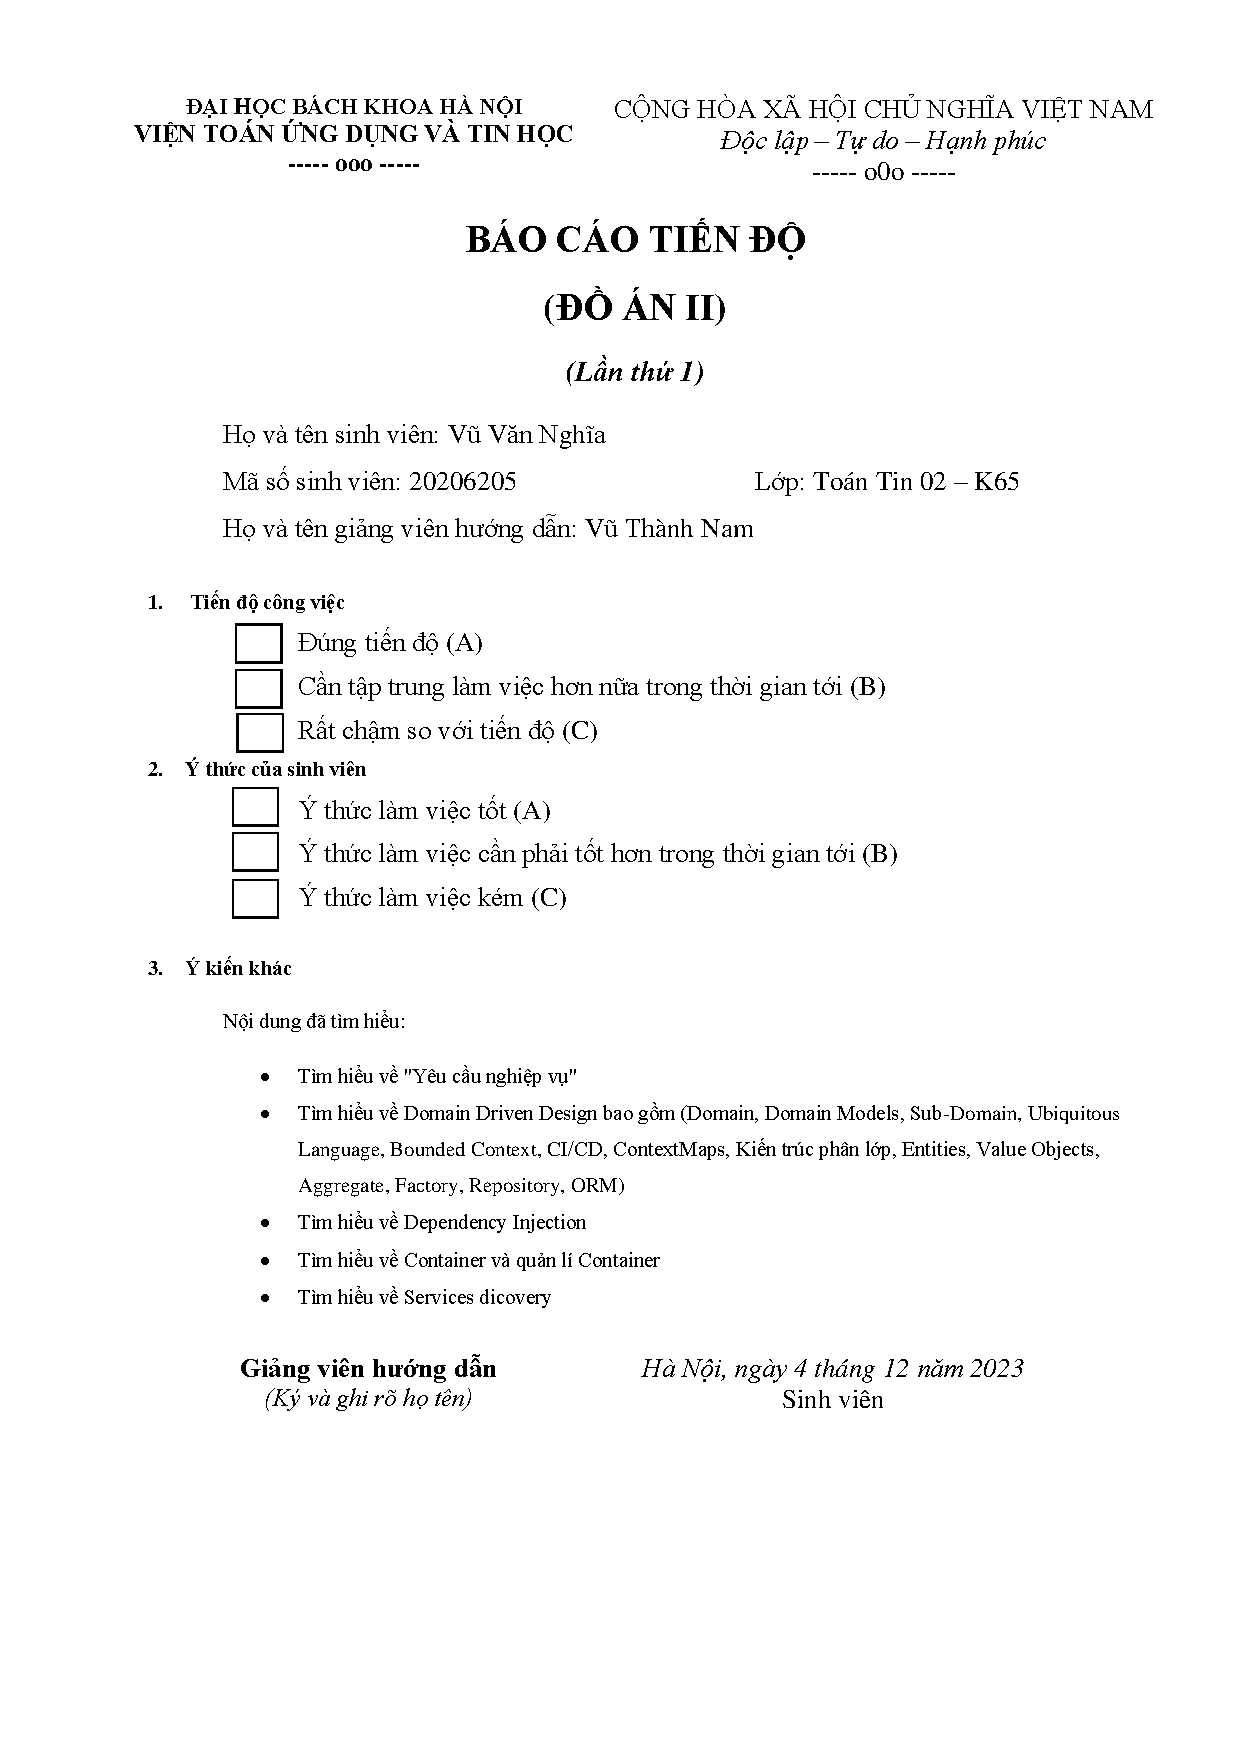
\includepdf[pages = -]{contents/bao_cao_tien_do/lan_1.pdf}
% 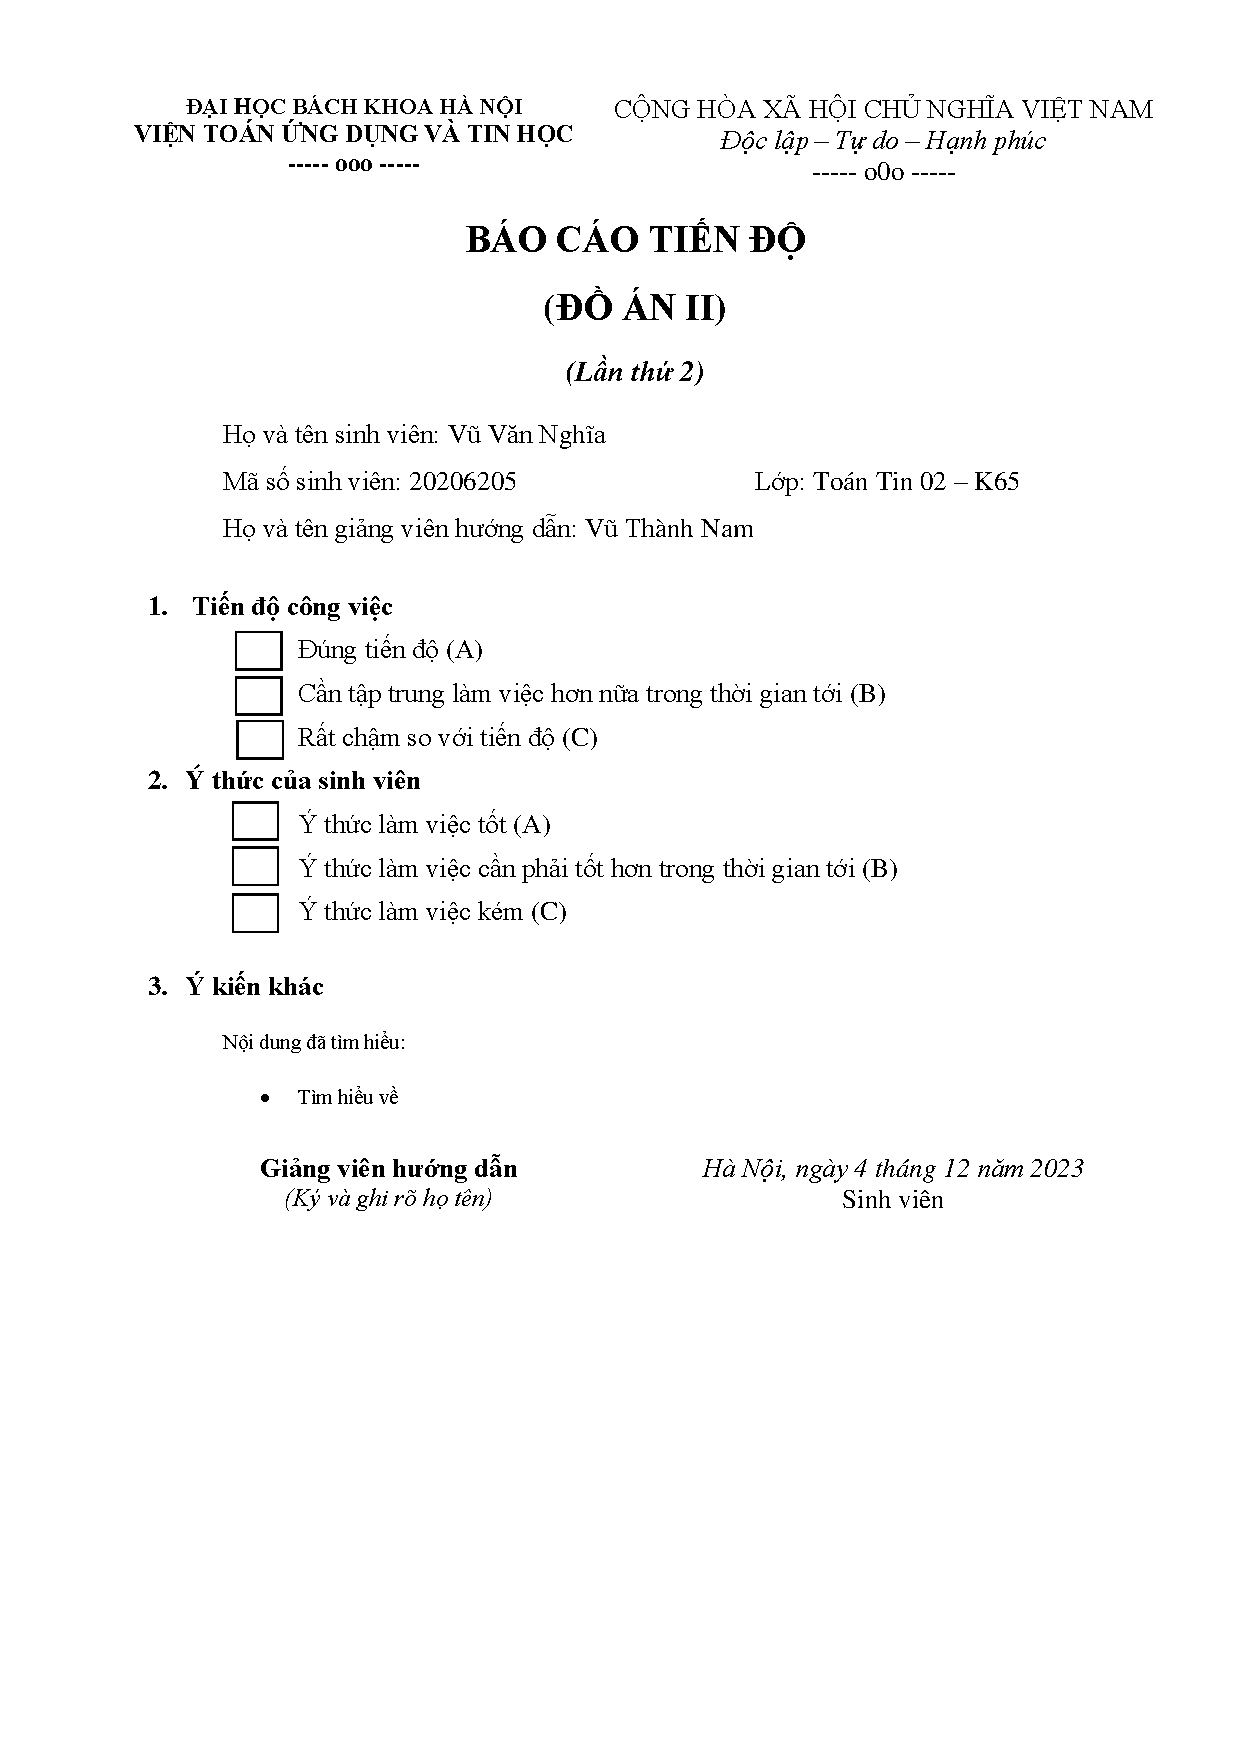
\includepdf[pages = -]{contents/bao_cao_tien_do/lan_2.pdf}
% \renewcommand*\contentsname{\centering MỤC LỤC}

\tableofcontents

\setcounter{page}{0}
% \chapter*{\centering LỜI CẢM ƠN}

\addcontentsline{toc}{chapter}{LỜI CẢM ƠN}

Trước hết, em xin gửi lời cảm ơn chân thành và sâu sắc đến TS. Vũ Thành Nam, người thầy đã tận tình hỗ trợ và hướng dẫn em suốt thời gian thực hiện đồ án. Những kiến thức và kinh nghiệm mà em đã tiếp thu được trong quá trình này sẽ đóng góp quan trọng vào sự phát triển và thành công của em trong tương lai. Em xin gửi lời chúc sức khỏe tốt nhất đến thầy, hy vọng thầy luôn dồi dào sức khỏe, đam mê và nhiệt huyết trong công việc giảng dạy.

Em cũng xin gửi lời cảm ơn tới các thầy cô giảng viên trong \emph{"Khoa Toán - Tin"} đã tận tình truyền đạt những kiến thức quý báu cho em. Những kiến thức này không chỉ giúp em phát triển về mặt tri thức mà còn nuôi dưỡng kỹ năng và đam mê trong quá trình học tập và nghiên cứu.

Trong quá trình hoàn thành bài báo cáo đồ án này không tránh khỏi những thiếu sót. Vì vậy, em mong nhận được sự giúp đỡ và ý kiến đóng góp chân thành từ các thầy cô để em có thể cải thiện một cách tốt nhất.

\emph{Em xin chân thành cảm ơn!}

\vspace{0.7cm}

\hspace{0.4\textwidth}\begin{minipage}{0.5\textwidth}

\noindent\begin{center}

\textit{Hà Nội, \today} \\

\vspace{0.5cm}

\textbf{Tác giả} \\

\vspace{0.5cm}

\textbf{Vũ Văn Nghĩa}

\end{center}

\end{minipage}
% \chapter*{\centering DANH SÁCH BẢNG}

\addcontentsline{toc}{chapter}{DANH SÁCH BẢNG}

\makeatletter

\renewcommand\listoftables{

\@starttoc{lot}

}

\makeatother

\listoftables
% \chapter*{\centering DANH SÁCH HÌNH ẢNH}

\addcontentsline{toc}{chapter}{DANH SÁCH HÌNH ẢNH}

\makeatletter

\renewcommand\listoffigures{

\@starttoc{lof}

}

\makeatother

\listoffigures
% # %%%%%%%%%%%%%%%%%%%%%%%%%%%%%%

%%%%%%%%%%%%%%%%%%%%%%%%%%%%%%

\chapter*{\centering DANH SÁCH CÁC CỤM TỪ VIẾT TẮT}

\addcontentsline{toc}{chapter}{DANH SÁCH CÁC CỤM TỪ VIẾT TẮT}

% @sau

% @sau

% @sau

% @sau

% @sau

% @sau

% @sau

% @sau

% @sau

% @sau

% @sau

% @sau

% @sau

% @sau

% @sau

% @sau

% @sau

% @sau

% @sau

% @sau

% @sau

% @sau

% @sau

% @sau

% @sau

% @sau

% @sau

% @sau

% @sau

% @sau

\begin{table}[h]

\centering

\begin{tabular}{|c|c|c|c|}

\hline

STT & Từ viết tắt & Từ viết đầy đủ & Mô tả \\

\hline

Dong1 & Dong1 & Cot1 & Cot2 \\

\hline

Dong2 & Dong2 & Cot1 & Cot2 \\

\hline

\end{tabular}

\end{table}

% API; Application Programming Interface; Giao diện lập trình ứng dụng

% CI/CD; Continuous Integration (CI) and Continuous Delivery (CD) ; Quá trình tích hợp và chuyển giao liên tục

% thiết kế hướng miền ; thiết kế hướng miền; Kỹ thuật thiết kế theo hướng miền

% DI; Dependency Injection; Cơ chế tiêm sự phụ thuộc giữa các đối tượng

% HTTP; Hypertext Transfer Protocol; Giao thức truyền tải siêu văn bản

% JSON; JavaScript Object Notation; Một kiểu dữ liệu mở rộng của JavaScript

% ORM; Object Relational Mapping; Một kỹ thuật ánh xạ các đối tượng lập trình với từng bảng trong CSDL quan hệ

% Cơ sở dữ liệu ; CSDL ;

% Tạo (Create), Đọc (Read), Sửa (Update), Xóa (Delete) ; CRUD ;

% Kubernetes ; K8s ; kubernetes

% Số điện thoại ; SĐT ;

% UML

% MVC; Model View Controller; Một mẫu thiết kế ứng dụng

% SQL

SOA; Service Oriented Architecture; Kiến trúc hướng dịch vụ

SOAP; Simple Object Access Protocol; Một giao thức để truy cập dịch vụ web

SPA; Single Page Application; Kiểu ứng dụng một trang

REST; Representational State Transfer; Một tiêu chuẩn thiết kế các API sử dụng cho các dịch vụ web

URL; Uniform Resource Locator ; Địa chỉ định vị tài nguyên trên Internet

XML; Extensible Markup Language; Ngôn ngữ đánh dấu mở rộng

% TCT ; TCT ;

Người nộp thuế ; NNT ;

Mã số thuế ; MST ;

Hóa đơn điện tử ; HĐĐT ;

Cơ quan thuế ; CQT ;

Công nghệ thông tin ; CNTT ;

%%%%%%%%%%%%%%%%%%%%%%%%%%%%%%
% # \chapter*{\centering DANH SÁCH CÁC THUẬT NGỮ}

\addcontentsline{toc}{chapter}{DANH SÁCH CÁC THUẬT NGỮ}

% @sau

% @sau

% @sau

% @sau

% @sau

% @sau

% @sau

% @sau

% @sau

% @sau

% @sau

% @sau

% @sau

% @sau

% @sau

% @sau

% @sau

% @sau

% @sau

% @sau

% @sau

% @sau

% @sau

% @sau

% @sau

% @sau

% @sau

% @sau

\begin{table}[h]

\centering

\begin{tabular}{|c|c|c|}

\hline

STT & Tiếng Anh & Tiếng Việt \\

\hline

Dong1 & Dong1 & Cot2 \\

\hline

Dong2 & Dong2 & Cot2 \\

\hline

\end{tabular}

\end{table}

% kiến trúc nguyên khối, kiến trúc nguyên khối

% kiến trúc nguyên khối, kiến trúc nguyên khối

% kiến trúc vi dịch, kiến trúc vi dịch

% kiến trúc vi dịch, kiến trúc vi dịch

% kiến trúc vi dịch, kiến trúc vi dịch

% kiến trúc vi dịch, kiến trúc vi dịch

% thiết kế hướng miền, thiết kế hướng miền

% thiết kế hướng miền, thiết kế hướng miền

1 thiết kế hướng miền

Thiết kế hướng lĩnh vực

2 Domain (không dịch)

3 Abstraction Trừu tượng

4 chuyên gia ngành
% \chapter*{\centering MỞ ĐẦU}
% \addcontentsline{toc}{chapter}{MỞ ĐẦU}
% \section*{Lý do chọn đề tài}
% Trong quá trình hoạt động kinh doanh, doanh nghiệp có nhu cầu chuyển đổi mô hình kinh doanh linh hoạt để có thể tồn tại và phát triển khi thị trường thay đổi. Từ đó, đáp ứng nhu cầu của khách hàng, mang lại ưu thế cạnh tranh so với các đối thủ.

Trong những năm gần đây, việc áp dụng kiến trúc vi dịch vụ ngày càng phổ biến, đem lại nhiều lợi ích như tách các nghiệp vụ kinh doanh thành các dịch vụ nhỏ độc lập, tăng tính linh hoạt và khả năng chống chịu sự cố của hệ thống.

Kiến trúc vi dịch vụ hỗ trợ doanh nghiệp chuyển đổi nhanh chóng để đáp ứng nhu cầu của mô hình kinh doanh và mong đợi của khách hàng. Tuy nhiên, để xây dựng được kiến trúc vi dịch vụ tốt, cần phải tạo ra các dịch vụ nhỏ phù hợp và duy trì tính độc lập. Trong đồ án này, em sử dụng thiết kế hướng miền để phân tích và xây dựng kiến trúc vi dịch vụ.

Theo quy định của Nghị định 123/2020/NĐ - CP, tất cả các doanh nghiệp, tổ chức và hộ kinh doanh đều bắt buộc phải sử dụng hóa điện tử. Vì vậy, nhu cầu sử dụng và xử lý hóa đơn điện tử trở nên rất lớn. Do đó trong đồ án này, em chọn chủ đề \emph{"Sử dụng thiết kế hướng miền xây dựng kiến trúc vi dịch vụ cho bài toán quản lý hóa đơn điện tử"}. Chủ đề này là một xu hướng quan trọng trong phát triển phần mềm và mang lại nhiều lợi ích trong việc cải thiện quá trình quản lý hóa đơn điện tử.
% \section*{Đối tượng và phạm vi nghiên cứu}
% % \begin{itemize}

\item \textbf{Đối tượng nghiên cứu:} Đối tượng nghiên cứu của đồ án này là phương pháp phát triển phần mềm theo hướng kiến trúc vi dịch vụ có sử dụng thiết kế hướng miền cùng các công nghệ liên quan như: xxxxxxxxxxxxxxxxx, xxxxxxxxxxxxxxxxx, xxxxxxxxxxxxxxxxx, xxxxxxxxxxxxxxxxx, xxxxxxxxxxxxxxxxx, xxxxxxxxxxxxxxxxx, xxxxxxxxxxxxxxxxx, xxxxxxxxxxxxxxxxx, \dots

#

\item \textbf{Phạm vi nghiên cứu:} Tìm hiểu thiết kế hướng miền xây dựng kiến trúc vi dịch vụ cho bài toán quản lý hóa đơn điện tử.

\end{itemize}
% \section*{Tóm tắt nội dung đồ án}
% % Báo cáo đồ án này được tổ chức thành các phần chính sau:
#
\begin{itemize}

\item \textbf{Chương 1: xxxxxxxxxxxxxxxxx}

\begin{quote}

xxxxxxxxxxxxxxxxx

\end{quote}

\item \textbf{Chương 1: xxxxxxxxxxxxxxxxx}

\begin{quote}

xxxxxxxxxxxxxxxxx

\end{quote}

\item \textbf{Chương 1: xxxxxxxxxxxxxxxxx}

\begin{quote}

xxxxxxxxxxxxxxxxx

\end{quote}

\end{itemize}

%@ Thêm các mục nhỏ như:

%@ Thêm các mục nhỏ như:

%@ Thêm các mục nhỏ như:

%@ Thêm các mục nhỏ như:

%@ Thêm các mục nhỏ như:

%@ Thêm các mục nhỏ như:

%@ Thêm các mục nhỏ như:

%@ Thêm các mục nhỏ như:

%@ Thêm các mục nhỏ như:

%@ Thêm các mục nhỏ như:

%@ Thêm các mục nhỏ như:

%@ Thêm các mục nhỏ như:

%@ Thêm các mục nhỏ như:

% Luận văn được tổ chức thành các phần chính sau:

% Mở đầu: Trình bày tổng quan về đề tài

% Chương 1: Trình bày cách thức phát triển phần mềm theo kiến trúc kiến trúc vi dịch vụ .

% Trong chương này, luận văn tập trung làm rõ các nội dung:

% - Sơ lược về một số hướng kiến trúc phần mềm truyền thống như kiến trúc nguyên

% khối, kiến trúc hướng dịch vụ, công nghệ ESB

% - Tổng quan về kiến trúc kiến trúc vi dịch vụ : sự ra đời, đặc điểm của kiến trúc vi dịch vụ

% - Các mẫu thiết kế quan trọng được sử dụng trong kiến trúc vi dịch vụ

% - Một số nguyên tắc thiết kế kiến trúc vi dịch vụ

% Chương 2: Trình bày hướng xây dựng ứng dụng web sử dụng micro - frontends.

% Trong chương này, luận văn tập trung làm rõ các nội dung:

% - Sơ lược về một số mô hình phát triển web như mô hình web tĩnh, mô hình web

% động, mô hình web theo hướng SPA

% - Sự ra đời của kiến trúc micro - frontends

% - Các cơ chế tích hợp micro - frontends được thảo luận như: tích hợp theo hướng

% “build - time”, tích hợp theo hướng “run - time”, cách thức điều hướng và giao tiếp

% giữa các micro - frontends

% Chương 3: Trình bày cách thức xây dựng một ứng dụng thử nghiệm sử dụng kiến

% trúc kiến trúc vi dịch vụ, micro - frontends. Một số nội dung chính trong quá trình thực nghiệm

% được làm rõ bao gồm:

% 3

% - Áp dụng phương pháp thiết kế hướng miền để phân hoạch, thiết kế chương trình

% - Thiết kế và cài đặt tầng dịch vụ theo hướng kiến trúc vi dịch vụ, sử dụng các công

% nghệ trên nền tảng Java như Spring Boot, Spring Cloud

% - Thiết kế và cài đặt tầng giao diện theo hướng micro - frontends, sử dụng các công

% nghệ như Single - SPA, Angular, ReactJS

% - Một số kỹ thuật kiểm thử kiến trúc vi dịch vụ cũng được thảo luận như kiểm thử đơn

% vị, kiểm thử tích hợp và kiểm thử mức giao diện

% - Cách thức triển khai ứng dụng sử dụng Docker

% Phần kết luận: Tổng kết, đánh giá kết quả thu được của quá trình nghiên cứu cũng

% như các ưu nhược điểm, các hạn chế và hướng phát triển tương lai.

% \chapter{Tổng quan về bài toán quản lý hóa đơn điện tử}
% Bài toán hóa đơn điện tử là một phần quan trọng của quá trình chuyển đổi số. Trong quá khứ, mọi người thường sử dụng hóa đơn giấy truyền thống. Ngày nay, khi có quy định kế toán và quản lý tài chính, hóa đơn điện tử đã trở nên phổ biến giúp giảm bớt sự phụ thuộc vào giấy tờ. Cùng với sự phát triển của khoa học công nghệ đã giúp quản lý hiệu quả công việc và tối ưu hóa quy trình kế toán và tài chính.
% \section{Các khái niệm và căn cứ pháp lý}
% \subsection{Hóa đơn}

\emph{Theo quy định tại khoản 1 Điều 3 Nghị định 123/2020/NĐ - CP:}

Hóa đơn là chứng từ kế toán do tổ chức, cá nhân bán hàng hóa, cung cấp dịch vụ lập, ghi nhận thông tin bán hàng hóa, cung cấp dịch vụ. Hóa đơn được thể hiện theo hình thức hóa đơn điện tử hoặc hóa đơn do cơ quan thuế đặt in.

\subsection{Hóa đơn điện tử}

\emph{Theo quy định tại khoản 2 Điều 3 Nghị định 123/2020/NĐ - CP:}

Hóa đơn điện tử là hóa đơn có mã hoặc không có mã của cơ quan thuế được thể hiện ở dạng dữ liệu điện tử do tổ chức, cá nhân bán hàng hóa, cung cấp dịch vụ lập bằng phương tiện điện tử để ghi nhận thông tin bán hàng hóa, cung cấp dịch vụ theo quy định của pháp luật về kế toán, pháp luật về thuế, bao gồm cả trường hợp hóa đơn được khởi tạo từ máy tính tiền có kết nối chuyển dữ liệu điện tử với cơ quan thuế, trong đó:

a. Hóa đơn điện tử có mã của cơ quan thuế là hóa đơn điện tử được cơ quan thuế cấp mã trước khi tổ chức, cá nhân bán hàng hóa, cung cấp dịch vụ gửi cho người mua. Mã của cơ quan thuế trên hóa đơn điện tử bao gồm số giao dịch là một dãy số duy nhất do hệ thống của cơ quan thuế tạo ra và một chuỗi ký tự được cơ quan thuế mã hóa dựa trên thông tin của người bán lập trên hóa đơn.

b. Hóa đơn điện tử không có mã của cơ quan thuế là hóa đơn điện tử do tổ chức bán hàng hóa, cung cấp dịch vụ gửi cho người mua không có mã của cơ quan thuế.

\subsection{Bắt buộc sử dụng hóa đơn điện tử từ 01/07/2022}

\emph{Theo quy định tại khoản 1 Điều 59 Nghị định 123/2020/NĐ - CP:}

Nghị định này có hiệu lực thi hành kể từ ngày 01 tháng 7 năm 2022, khuyến khích cơ quan, tổ chức, cá nhân đáp ứng điều kiện về hạ tầng công nghệ thông tin áp dụng quy định về hóa đơn, chứng từ điện tử của Nghị định này trước ngày 01 tháng 7 năm 2022.

$\Rightarrow$ Theo quy định, tất cả các doanh nghiệp, tổ chức và hộ kinh doanh đều bắt buộc phải chuyển từ sử dụng hóa đơn giấy sang hóa đơn điện tử bắt đầu từ tháng 07/2022. Vì vậy, nhu cầu sử dụng và xử lý hóa đơn điện tử trở nên rất cần thiết. Do đó ở đồ án này, em chọn chủ đề về quản lý hóa đơn điện tử.

\subsection{Qui định lưu trữ hóa đơn điện tử}

\emph{Theo quy định tại khoản 1 Điều 11 Thông tư 32/2011/TT - BTC:}

Người bán, người mua hàng hoá, dịch vụ sử dụng hóa đơn điện tử để ghi sổ kế toán, lập báo cáo tài chính phải lưu trữ hóa đơn điện tử theo thời hạn quy định của Luật Kế toán. Trường hợp hóa đơn điện tử được khởi tạo từ hệ thống của tổ chức trung gian cung cấp giải pháp hóa đơn điện tử thì tổ chức trung gian này cũng phải thực hiện lưu trữ hóa đơn điện tử theo thời hạn nêu trên.

\emph{Theo quy định tại khoản 5 Điều 41 Luật số 88/2015/QH13:}

1. Tài liệu kế toán phải được lưu trữ theo thời hạn sau đây:

a. Ít nhất là 05 năm đối với tài liệu kế toán dùng cho quản lý, điều hành của đơn vị kế toán, gồm cả chứng từ kế toán không sử dụng trực tiếp để ghi sổ kế toán và lập báo cáo tài chính.

b. Ít nhất là 10 năm đối với chứng từ kế toán sử dụng trực tiếp để ghi sổ kế toán và lập báo cáo tài chính, sổ kế toán và báo cáo tài chính năm, trừ trường hợp pháp luật có quy định khác.

c. Lưu trữ vĩnh viễn đối với tài liệu kế toán có tính sử liệu, có ý nghĩa quan trọng về kinh tế, an ninh, quốc phòng.

$\Rightarrow$ Như vậy, hóa đơn điện tử sẽ được lưu trữ trên hệ thống hóa đơn điện tử của nhà cung cấp hoặc doanh nghiệp với thời gian lưu trữ ít nhất là 10 năm theo quy định của pháp luật.

\subsection{Một số lợi ích của hóa đơn điện tử}

\emph{Một số lợi ích của hóa đơn điện tử:}

\begin{itemize}

\item Tuân thủ các quy định về thuế và pháp luật.

\item Thể hiện tính minh bạch: bảo vệ quyền lợi của người mua và người bán.

\item Giúp tiết kiệm chi phí in ấn, lưu trữ và bảo quản.

\item Loại bỏ rủi ro cháy, hỏng hoặc mất và dễ dàng sao lưu.

\item Dễ dàng tra cứu, phát hành, quản lý, tạo báo cáo và giảm thủ tục giấy tờ.

\item Giúp theo dõi tình hình tài chính của công ty (doanh thu, chi phí, lợi nhuận).

\end{itemize}
% \section{Yêu cầu nghiệp vụ}
% Yêu cầu nghiệp vụ là phần nội dung quan trọng xác định nội dung, phạm vi, mục tiêu và chức năng mong muốn của hệ thống. Giúp hệ thống đáp ứng đúng mục đích và nhu cầu kinh doanh. Ngoài ra, yêu cầu nghiệp vụ là yếu tố quan trọng trong thiết kế hướng miền vì thiết kế hướng miền là một phương pháp thiết kế phần mềm tập trung vào việc hiểu và mô hình hóa \emph{lĩnh vực kinh doanh}.
% \subsection{Yêu cầu nghiệp vụ của bài toán phụ}
% Trang web \emph{"https://hoadondientu.gdt.gov.vn"} là trang web do Tổng cục Thuế quản lý và sử dụng để thực hiện các quy trình liên quan đến thuế điện tử. Thực tế, yêu cầu đăng ký và phê duyệt chính thức từ Tổng cục Thuế dành cho cá nhân và doanh nghiệp. Trong đồ án này, em sẽ tạo một phiên bản giả lập của hệ thống chính thức là \emph{"tct-demo"}, dành cho mục đích học tập phục vụ cho bài toán chính là \emph{"Xây dựng kiến trúc vi dịch vụ cho bài toán hóa đơn điện tử"}.
% \subsection{Yêu cầu nghiệp vụ của bài toán chính}
% \subsubsection{Các chức năng thay đổi so với thực tế trong đồ án này}
% Để đơn giản bài toán, các chức năng trong đồ án này đã thay đổi so với bài toán thực tế như sau:

\begin{itemize}

\item Bỏ qua định dạng tập tin của hóa đơn

\begin{itemize}

\item Trong đồ án này, em bỏ qua định dạng tập tin của hóa đơn ví dụ: XML, PDF, EXCEL, \dots

\end{itemize}

\item Thay đổi phần mã số thuế và chữ ký số

\begin{itemize}

\item Mã số thuế được tạo khi sau đăng ký phần mềm quản lý hóa đơn điện tử.

\begin{itemize}

\item Trong thực tế, cơ quan thuế quản lý mã số thuế có 10 ký tự đại diện cá nhân, doanh nghiệp hoặc 14 ký tự đại diện chi nhánh của doanh nghiệp.

% Người nộp thuế dùng mã số thuế gửi đăng ký tới Tổng cục Thuế theo 2 cách:

% \item Trong thực tế, cơ quan thuế quản lý mã số thuế có 10 ký tự đại diện cá nhân, doanh nghiệp hoặc 14 ký tự đại diện chi nhánh của doanh nghiệp. Người nộp thuế dùng mã số thuế gửi đăng ký tới Tổng cục Thuế theo 2 cách:

% \begin{itemize}

% \item Đăng ký qua tổ chức cung cấp dịch vụ quản lý hóa đơn điện tử.

% \item Đăng ký trên cổng thông tin điện tử của Tổng cục Thuế.

% \end{itemize}

\item Trong đồ án này, khi người nộp thuế đăng ký tài khoản của phần mềm quản lý hóa đơn điện tử, mã số thuế được tạo bằng cách phần mềm quản lí hóa đơn gửi yêu cầu đến tct-demo.

\end{itemize}

\item Bỏ qua phần chữ ký số.

% thay thế bằng ứng dụng xác thực.

\begin{itemize}

\item Trong thực tế, chữ ký số của mọi doanh nghiệp là USB Token. Trong đồ án này, em xin phép bỏ qua phần chữ ký số.

% thay thế chữ ký số bằng ứng dụng xác thực 2 yếu tố sau khi đăng nhập phần mềm quản lý hóa đơn điện tử.

% \item Trong đồ án này, em thay thế chữ ký số bằng ứng dụng xác thực 2 yếu tố sau khi đăng nhập phần mềm quản lý hóa đơn điện tử.

% \begin{example} Ứng dụng xác thực như Google Authenticator, Microsoft Authenticator, \dots

% \end{example}

\end{itemize}

\end{itemize}

% \item Bỏ qua phần ký hiệu hóa đơn

% % https://www.meinvoice.vn/tin-tuc/12961/mau-so-hoa-don-va-ky-hieu-hoa-don-dien-tu-nd123-tt78

\item Bỏ qua chức năng lập hóa đơn điều chỉnh

\begin{itemize}

\item Trong đồ án này, em bỏ qua chức năng lập hóa đơn điều chỉnh và chỉ có chức năng lập hóa đơn thay thế (sửa hóa đơn).

\end{itemize}

\item Bỏ qua chức năng phê duyệt hóa đơn

\item Bỏ qua chức năng đa người thuê (multi-tenancy)

\begin{itemize}

\item Trong đồ án này, em bỏ qua chức năng đa người thuê, đối với 1 người nộp thuế chỉ có 1 tài khoản tương tác quản lý hóa đơn điện tử.

% (multi-tenancy) và chỉ có chức năng đơn người thuê (single-tenancy).







% Chỉ dùng 1 loại hóa đơn vì em thấy tương tự.

% Loại hóa đơn: + Hóa đơn giá trị gia tăng + Hóa đơn bán hàng + Hóa đơn bán tài sản công + Hóa đơn bán hàng dự trữ quốc gia + Hóa đơn khác + Chứng từ điện tử được sử dụng và quản lý như hóa đơn
\end{itemize}

\end{itemize}
% \subsubsection{Các chức năng tổng quan của bài toán chính}
% Các chức năng của bài toán chính quản lí hóa đơn bao gồm:
\begin{itemize}



\item Quản lý tài khoản
\begin{itemize}
    \item Đăng ký, Đăng nhập, Đăng xuất, Quên mật khẩu, Đổi mật khẩu, Thay đổi thông tin
\end{itemize}


\item Quản lý danh mục

\begin{itemize}

\item Quản lý khách hàng

\item Quản lý hàng hóa, dịch vụ

\end{itemize}




\item Quản lý hóa đơn

\begin{itemize}

\item Thêm hóa đơn, Sửa hóa đơn, Xóa hóa đơn

\end{itemize}



\item Tra cứu hóa đơn

Có 3 cách tra cứu:

\begin{itemize}

\item Tra cứu hóa đơn theo số hóa đơn

\item Tra cứu tất cả hóa đơn bán ra

\item Tra cứu tất cả hóa đơn mua vào

\end{itemize}



\item Báo cáo thống kê

\begin{itemize}

\item Số lượng hóa đơn bán ra

\item Số lượng hóa đơn mua vào

\item Số lượng khách hàng

\item Số lượng sản phẩm

\item Thông tin về chi phí

\item Thông tin về lợi nhuận

\item Thông tin về thuế

\end{itemize}

\end{itemize}

\end{document}


 
 


\item Thông báo

Có chức năng tìm kiếm chi tiết, tìm kiếm tất cả, thêm, sửa, xóa đối với thông báo có các thông tin:

\begin{itemize}

\item Mã, Tiêu đề, Nội dung, Thời gian

\end{itemize}

\item Thư điện tử

\begin{itemize}

\item Chức năng này giúp gửi thông tin hóa đơn cho khách hàng.

\end{itemize}

\item Quản lý hệ thống

Tương tự như bài toán phụ nhưng có thêm quyền:

\begin{itemize}

\item Thông báo

\item Thư điện tử

\end{itemize}

\end{itemize}

% % Chi tiết các chức năng của bài toán chính quản lí hóa đơn bao gồm:

% \begin{itemize}

% \item Quản lý tài khoản

% \begin{itemize}

% \item Đăng ký

% \begin{itemize}

% \item Người nộp thuế nhập các thông tin:

% \begin{itemize}

% \item Email, Mật khẩu, Họ tên, Số điện thoại, Địa chỉ

% % \item Mã số thuế có 10 ký tự đại diện cá nhân, doanh nghiệp hoặc 14 ký tự đại diện chi nhánh của doanh nghiệp với định dạng "Mã số thuế doanh nghiệp-Mã chi nhánh". %# Code "Mã số thuế phải có độ dài 10 hoặc 14 ký tự và đúng định dạng."

% % Mã số thuế 10 ký tự: 0123456789

% % Mã số thuế 14 ký tự: 0123456789-001

% % \item Nếu mã số thuế đã tồn tại đăng ký, hệ thống sẽ thông báo: "Mã số thuế đã đăng ký sử dụng hóa đơn điện tử." %# Code

% % \item Người liên hệ: phải chứa một chuỗi kí tự tên hợp lệ, không có số và không được để trống. %# Code

% % \item Điện thoại liên hệ: phải chứa một chuỗi kí tự số và dấu "+" ở đầu (nếu có) và không được để trống. %# Code

% % \item Địa chỉ liên hệ: phải chứa một chuỗi kí tự địa chỉ hợp lệ và không được để trống. %# Code

% % \item Thư điện tử: phải chứa một chuỗi kí tự có định dạng email và không được để trống. %# Code

% \end{itemize}

% \item Tiếp theo, người nộp thuế chọn hình thức hóa đơn: %# Code enum

% \begin{itemize}

% \item Hóa đơn có mã của cơ quan thuế

% \item Hóa đơn không có mã của cơ quan thuế

% \end{itemize}

% \item Cuối cùng, người nộp thuế gửi đăng ký với thời gian đang thực hiện đăng ký.

% %# Code "Gửi thông tin đăng ký hóa đơn điện tử cho cơ quan thuế thành công."

% %# Code "Gửi thông tin đăng ký hóa đơn điện tử cho cơ quan thuế thành công."

% \end{itemize}

% \item Đăng nhập

% \begin{itemize}

% \item Sau khi đăng ký thành công, người nộp thuế nhận được thông tin đăng nhập tài khoản của quản trị viên qua email bao gồm: Tên người dùng và Mật khẩu

% % Tên người dùng xxxxx.admin

% % \item Nếu thông tin đăng nhập không chính xác, hệ thống sẽ thông báo: "Thông tin đăng nhập không chính xác." %# Code

% \item Người nộp thuế thực hiện đăng nhập và tạo chữ ký số.

% \end{itemize}

% \item Đăng xuất

% \begin{itemize}

% \item Thực hiện chức năng đăng xuất tài khoản.

% \end{itemize}

% \item Quên mật khẩu

% \begin{itemize}

% \item \emph{Chức năng quên mật khẩu chỉ áp dụng cho tài khoản của quản trị viên. Đối với loại tài khoản khác, người dùng cần liên hệ quản trị viên.}

% \item Quản trị viên cung cấp tên đăng nhập.

% \item Quản trị viên dùng chữ ký số để gửi yêu cầu khôi phục mật khẩu.

% \item $\Rightarrow$ \emph{Sau khi gửi yêu cầu, quản trị viên sẽ nhận được mật khẩu mới qua thư điện tử.}

% %# Code "Gửi yêu cầu khôi phục mật khẩu thành công."

% \end{itemize}

% \item Đổi mật khẩu

% \begin{itemize}

% \item Để thay đổi mật khẩu cần cung cấp thông tin:

% \begin{itemize}

% \item Mật khẩu cũ, Mật khẩu mới, Nhập lại mật khẩu mới

% \end{itemize}

% % \begin{vmatrix}

% % \begin{itemize}

% % \item Mật khẩu: phải chứa một chuỗi có độ dài lớn hơn 8 kí tự và không được để trống. %# Code

% % \item Nếu mật khẩu cũ không chính xác, hệ thống sẽ thông báo: "Mật khẩu cũ không chính xác." %# Code

% % \item Nếu mật khẩu mới không trùng khớp, hệ thống sẽ thông báo: "Mật khẩu mới không trùng khớp." %# Code

% % \end{itemize}

% % \end{vmatrix}

% \end{itemize}

% \item Thay đổi thông tin

% \begin{itemize}

% \item Trong quá trình sử dụng hóa đơn điện tử, người nộp thuế có thể thay đổi thông tin:

% \begin{itemize}

% \item Tên người nộp thuế, Người liên hệ, Điện thoại liên hệ, Địa chỉ liên hệ, Thư điện tử

% \end{itemize}

% \begin{vmatrix}

% \begin{itemize}

% \item Tên người nộp thuế: phải chứa một chuỗi kí tự tên hợp lệ, không có số và không được để trống. %# Code

% \item Người liên hệ: phải chứa một chuỗi kí tự tên hợp lệ, không có số và không được để trống. %# Code

% \item Điện thoại liên hệ: phải chứa một chuỗi kí tự số và dấu "+" ở đầu (nếu có) và không được để trống. %# Code

% \item Địa chỉ liên hệ: phải chứa một chuỗi kí tự địa chỉ hợp lệ và không được để trống. %# Code

% \item Thư điện tử: phải chứa một chuỗi kí tự có định dạng email và không được để trống. %# Code

% \end{itemize}

% \end{vmatrix}

% \item Sau đó, người nộp thuế dùng chữ ký số để xác nhận gửi thay đổi với ngày thực hiện là ngày đang thay đổi thông tin.

% $\Rightarrow$ \emph{Sau khi gửi thay đổi, người nộp thuế sẽ nhận được thông báo của cơ quan thuế qua thư điện tử về việc tiếp nhận và chấp nhận thay đổi.} %# Code "Gửi thông tin thay đổi hóa đơn điện tử cho cơ quan thuế thành công."

% \end{itemize}

% \end{itemize}

% \item Quản lý danh mục

% \begin{itemize}

% \item Quản lý khách hàng

% Có chức năng tìm kiếm chi tiết, tìm kiếm tất cả, thêm, sửa, xóa đối với khách hàng có các thông tin:

% \begin{itemize}

% \item Mã, Tên, Mã số thuế, Địa chỉ, Số điện thoại, Số tài khoản, Ngân hàng

% \end{itemize}

% \begin{vmatrix}

% \begin{itemize}

% \item Tên: phải chứa một chuỗi kí tự tên hợp lệ, không có số và không được để trống. %# Code

% \item Mã số thuế: 10 ký tự đại diện cá nhân, doanh nghiệp hoặc 14 ký tự đại diện chi nhánh của doanh nghiệp với định dạng "Mã số thuế doanh nghiệp-Mã chi nhánh". % # Code

% \item Địa chỉ: phải chứa một chuỗi kí tự địa chỉ hợp lệ và không được để trống. % # Code

% \item Số điện thoại: phải chứa một chuỗi kí tự số và dấu "+" ở đầu (nếu có) và không được để trống. % # Code

% \item Số tài khoản: phải chứa một chuỗi kí tự và không được để trống. % # Code

% \item Ngân hàng: phải chứa một chuỗi kí tự ngân hàng hợp lệ và không được để trống. % # Code

% \end{itemize}

% \end{vmatrix}

% \item Quản lý hàng hóa, dịch vụ

% Có chức năng tìm kiếm chi tiết, tìm kiếm tất cả, thêm, sửa, xóa đối với hàng hóa, dịch vụ có các thông tin:

% \begin{itemize}

% \item Mã, Tên, Đơn vị tính, Đơn giá, Thuế suất, Ghi chú

% \end{itemize}

% \begin{vmatrix}

% \begin{itemize}

% \item Tên: phải chứa một chuỗi kí tự và không được để trống. %# Code

% \item Đơn vị tính: phải chứa một chuỗi kí tự và không được để trống. %# Code

% \item Đơn giá: phải có định dạng là số. %# Code

% \item Thuế suất: phải có định dạng là số. %# Code

% \item Ghi chú: nội dung không bắt buộc. %# Code

% \end{itemize}

% \end{vmatrix}

% \end{itemize}

% \item Quản lý hóa đơn

% \begin{itemize}

% \item Thêm hóa đơn

% \begin{itemize}

% \item Nhập thông tin người bán:

% \begin{itemize}

% \item Tên, Mã số thuế, Địa chỉ, Số điện thoại, Số tài khoản, Ngân hàng

% \end{itemize}

% \item Nhập thông tin người mua:

% \begin{itemize}

% \item Tên, Mã số thuế, Địa chỉ, Số điện thoại, Số tài khoản, Ngân hàng

% \end{itemize}

% \item Nhập thông tin hàng hóa, dịch vụ:

% \begin{itemize}

% \item Tên, Đơn vị tính, Đơn giá, Số lượng, Thuế suất, Ghi chú

% \end{itemize}

% \item Hệ thống tự động tính toán:

% \begin{itemize}

% \item Số hóa đơn

% \item Ngày lập hóa đơn

% \item Tổng tiền trước thuế

% \item Tổng tiền sau thuế

% \end{itemize}

% \end{itemize}

% \item Sửa hóa đơn

% \begin{itemize}

% \item Chức năng này cho phép thay đổi các thông tin trong hóa đơn.

% \item Hệ thống cần lưu trữ lịch sử thay đổi của hóa đơn.

% \end{itemize}

% % % Lưu ý:

% % % - Hãy lưu trữ thông tin ID của hóa đơn thay thế trong trạng thái "Bị thay thế" của hóa đơn gốc.

% % % - Hãy lưu trữ thông tin ID của hóa đơn gốc trong trạng thái "Thay thế" của hóa đơn thay thế.

% \item Xóa hóa đơn

% \begin{itemize}

% \item Chức năng này cho phép xóa hóa đơn.

% \end{itemize}

% \end{itemize}

% \item Tra cứu hóa đơn

% \begin{itemize}

% \item Tra cứu khi chưa đăng nhập

% \begin{itemize}

% \item Tra cứu hóa đơn

% \begin{itemize}

% \item Người tra cứu nhập thông tin bao gồm: mã số thuế người bán, số hóa đơn, tổng tiền sau thuế.

% \end{itemize}

% \textbf{Kết quả:}

% \begin{itemize}

% \item Nếu thông tin hóa đơn không hợp lệ, hệ thống sẽ thông báo: "Không tồn tại hóa đơn có thông tin trùng khớp với các thông tin tổ chức, cá nhân tìm kiếm." %# Code

% \item Nếu thông tin hóa đơn hợp lệ, hệ thống sẽ thông báo: "Tồn tại hóa đơn có thông tin trùng khớp với các thông tin tổ chức, cá nhân tìm kiếm." %# Code

% \item Nếu hóa đơn là hóa đơn thay thế, bị thay thế hệ thống sẽ hiển thị thông tin bổ sung về hóa đơn liên quan: "Hóa đơn này là hóa đơn thay thế cho hóa đơn có số hóa đơn là: \textbf{số hóa đơn}." hoặc "Hóa đơn này là hóa đơn bị thay thế của hóa đơn có có số hóa đơn là: \textbf{số hóa đơn}." %# Code

% \end{itemize}

% \item Tra cứu mã số thuế

% \begin{itemize}

% \item Người tra cứu nhập mã số thuế.

% \end{itemize}

% \textbf{Kết quả:}

% \begin{itemize}

% \item Nếu đã đăng kí, hệ thống sẽ hiển thị thông báo: "Mã số thuế: \textbf{mã số thuế} đã đăng ký sử dụng hóa đơn điện tử theo Nghị định 123/2020/NĐ - CP." %# Code

% \item Nếu NNT chưa đăng kí, hệ thống sẽ hiển thị thông báo: "Mã số thuế: \textbf{mã số thuế} chưa sử dụng hóa đơn điện tử theo Nghị định 123/2020/NĐ - CP." %# Code

% \end{itemize}

% \end{itemize}

% \item Tra cứu khi đã đăng nhập

% \begin{itemize}

% \item Hệ thống hỗ trợ tra cứu 2 loại hóa đơn là hóa đơn bán ra và hóa đơn mua vào.

% \end{itemize}

% \end{itemize}

% \item Quản lý hệ thống

% \begin{itemize}

% \item Quản lý vai trò

% \begin{itemize}

% \item Người quản trị là một vai trò cố định có quyền sử dụng tất cả các chức năng.

% \item Người quản trị có thể thực hiện chức năng tìm kiếm chi tiết, tìm kiếm tất cả, thêm, sửa, xóa đối với vai trò:

% \begin{itemize}

% \item Tên vai trò

% \item Quyền

% \end{itemize}

% \end{itemize}

% \begin{vmatrix}

% \begin{itemize}

% \item Tên vai trò: phải chứa một chuỗi kí tự và không được để trống. %# Code

% \item Các quyền trong hệ thống bao gồm: %# Code

% \begin{itemize}

% \item Thay đổi thông tin người nộp thuế

% \item Quản lý khách hàng

% \item Quản lý hàng hóa, dịch vụ

% \item Thêm hóa đơn

% \item Sửa hóa đơn

% \item Xóa hóa đơn

% \item Tra cứu hóa đơn

% \end{itemize}

% \end{itemize}

% \end{vmatrix}

% \item Quản lý người dùng

% \begin{itemize}

% \item Người quản trị có thể thực hiện chức năng tìm kiếm chi tiết, tìm kiếm tất cả, thêm, sửa, xóa đối với người dùng:

% \begin{itemize}

% \item Tên đăng nhập

% \item Mật khẩu

% \item Vai trò

% \end{itemize}

% \end{itemize}

% \begin{vmatrix}

% \begin{itemize}

% \item Tên đăng nhập: phải chứa một chuỗi kí tự với định dạng "Mã số thuế.Tên đăng nhập" và không được để trống. %# Code

% \begin{example}

% Tên đăng nhập: 0123456789.vvn20206205

% \end{example}

% \item Mật khẩu: phải chứa một chuỗi có độ dài lớn hơn 8 kí tự và không được để trống. %# Code

% \item Vai trò: là vai trò được người quản trị đã tạo. %# Code

% \end{itemize}

% \end{vmatrix}

% \end{itemize}

% \item Gửi thông tin làm việc của Tổng cục Thuế qua thư điện tử cho người nộp thuế.

% \end{itemize}

% % Các chức năng tổng quan của bài toán phụ bao gồm:

% % Các chức năng tổng quan của bài toán phụ bao gồm:

% % Các chức năng tổng quan của bài toán phụ bao gồm:

% % Các chức năng tổng quan của bài toán phụ bao gồm:

% % Các chức năng tổng quan của bài toán phụ bao gồm:

% % Các chức năng tổng quan của bài toán phụ bao gồm:

% % Các chức năng tổng quan của bài toán phụ bao gồm:

% % Các chức năng tổng quan của bài toán phụ bao gồm:

% % Các chức năng tổng quan của bài toán phụ bao gồm:

% % Các chức năng tổng quan của bài toán phụ bao gồm:

% % Các chức năng tổng quan của bài toán phụ bao gồm:

% % Các chức năng tổng quan của bài toán phụ bao gồm:

% % Các chức năng tổng quan của bài toán phụ bao gồm:

% % Các chức năng tổng quan của bài toán phụ bao gồm:

% % Các chức năng tổng quan của bài toán phụ bao gồm:

% % Các chức năng tổng quan của bài toán phụ bao gồm:

% % Các chức năng tổng quan của bài toán phụ bao gồm:

% % Các chức năng tổng quan của bài toán phụ bao gồm:

% % Các chức năng tổng quan của bài toán phụ bao gồm:

% % Các chức năng tổng quan của bài toán phụ bao gồm:

% % Các chức năng tổng quan của bài toán phụ bao gồm:

% % Các chức năng tổng quan của bài toán phụ bao gồm:

% \begin{itemize}

% \item Quản lý tài khoản

% \begin{itemize}

% \item Đăng ký, Đăng nhập, Đăng xuất, Quên mật khẩu, Đổi mật khẩu, Thay đổi thông tin

% \end{itemize}

% \item Quản lý danh mục

% \begin{itemize}

% \item Quản lý khách hàng

% \item Quản lý hàng hóa, dịch vụ

% \end{itemize}

% \item Quản lý hóa đơn

% \begin{itemize}

% \item Thêm hóa đơn, Sửa hóa đơn, Xóa hóa đơn

% \end{itemize}

% \item Tra cứu hóa đơn

% \begin{itemize}

% \item Tra cứu khi chưa đăng nhập

% \begin{itemize}

% \item Tra cứu hóa đơn

% \item Tra cứu mã số thuế

% \end{itemize}

% \item Tra cứu khi đã đăng nhập

% \begin{itemize}

% \item Tra cứu hóa đơn mua vào.

% \item Tra cứu hóa đơn bán ra.

% \end{itemize}

% \end{itemize}

% \item Quản lý hệ thống

% \begin{itemize}

% \item Quản lý vai trò

% \item Quản lý người dùng

% \end{itemize}

% \item Gửi thông tin làm việc của Tổng cục Thuế qua thư điện tử cho người nộp thuế.

% \end{itemize}

% % Yêu cầu nghiệp vụ của bài toán chính phần mềm quản lí hóa đơn bao gồm:

% % Yêu cầu nghiệp vụ của bài toán chính phần mềm quản lí hóa đơn bao gồm:

% % Yêu cầu nghiệp vụ của bài toán chính phần mềm quản lí hóa đơn bao gồm:

% % Yêu cầu nghiệp vụ của bài toán chính phần mềm quản lí hóa đơn bao gồm:

% % Yêu cầu nghiệp vụ của bài toán chính phần mềm quản lí hóa đơn bao gồm:

% % Yêu cầu nghiệp vụ của bài toán chính phần mềm quản lí hóa đơn bao gồm:

% % Yêu cầu nghiệp vụ của bài toán chính phần mềm quản lí hóa đơn bao gồm:

% % Yêu cầu nghiệp vụ của bài toán chính phần mềm quản lí hóa đơn bao gồm:

% % Yêu cầu nghiệp vụ của bài toán chính phần mềm quản lí hóa đơn bao gồm:

% % Yêu cầu nghiệp vụ của bài toán chính phần mềm quản lí hóa đơn bao gồm:

% % Yêu cầu nghiệp vụ của bài toán chính phần mềm quản lí hóa đơn bao gồm:

% % Yêu cầu nghiệp vụ của bài toán chính phần mềm quản lí hóa đơn bao gồm:

% % Yêu cầu nghiệp vụ của bài toán chính phần mềm quản lí hóa đơn bao gồm:

% % Yêu cầu nghiệp vụ của bài toán chính phần mềm quản lí hóa đơn bao gồm:

% % Yêu cầu nghiệp vụ của bài toán chính phần mềm quản lí hóa đơn bao gồm:

% % Yêu cầu nghiệp vụ của bài toán chính phần mềm quản lí hóa đơn bao gồm:

% % Yêu cầu nghiệp vụ của bài toán chính phần mềm quản lí hóa đơn bao gồm:

% % Yêu cầu nghiệp vụ của bài toán chính phần mềm quản lí hóa đơn bao gồm:

% % Yêu cầu nghiệp vụ của bài toán chính phần mềm quản lí hóa đơn bao gồm:

% % Yêu cầu nghiệp vụ của bài toán chính phần mềm quản lí hóa đơn bao gồm:

% \begin{itemize}

% \item Quản lý tài khoản

% Tương tự như bài toán phụ.

% \item Quản lý danh mục

% Tương tự như bài toán phụ.

% \item Quản lý hóa đơn

% Tương tự như bài toán phụ.

% \item Tra cứu hóa đơn

% Có 3 cách tra cứu:

% \begin{itemize}

% \item Tra cứu hóa đơn theo số hóa đơn

% \item Tra cứu tất cả hóa đơn bán ra

% \item Tra cứu tất cả hóa đơn mua vào

% \end{itemize}

% \item Báo cáo thống kê

% \begin{itemize}

% \item Số lượng hóa đơn bán ra

% \item Số lượng hóa đơn mua vào

% \item Số lượng khách hàng

% \item Số lượng sản phẩm

% \item Thông tin về chi phí

% \item Thông tin về lợi nhuận

% \item Thông tin về thuế

% \end{itemize}

% \item Thông báo

% Có chức năng tìm kiếm chi tiết, tìm kiếm tất cả, thêm, sửa, xóa đối với thông báo có các thông tin:

% \begin{itemize}

% \item Mã, Tiêu đề, Nội dung, Thời gian

% \end{itemize}

% \item Thư điện tử

% \begin{itemize}

% \item Chức năng này giúp gửi thông tin hóa đơn cho khách hàng.

% \end{itemize}

% \item Quản lý hệ thống

% Tương tự như bài toán phụ nhưng có thêm quyền:

% \begin{itemize}

% \item Thông báo

% \item Thư điện tử

% \end{itemize}

% \end{itemize}

% % SAU

% % \item Người nộp thuế chọn loại hóa đơn: %# Code enum

% % \begin{itemize}

% % \item Hóa đơn điện tử giá trị gia tăng

% % \item Hóa đơn bán hàng

% % \item Hóa đơn bán tài sản công

% % \item Hóa đơn bán hàng dự trữ quốc gia

% % \item Hóa đơn khác

% % \end{itemize}

% \chapter{Giới thiệu về kiến trúc vi dịch vụ}
% Trong quá trình hoạt động kinh doanh, không phải mọi doanh nghiệp đều giữ nguyên mô hình kinh doanh được đưa ra ban đầu. Việc chuyển đổi mô hình kinh doanh là điều cần thiết, giúp các doanh nghiệp có thể phát triển linh hoạt và tồn tại.

\begin{example}

\begin{itemize}

\item Google bắt đầu như công cụ tìm kiếm trực tuyến, nhưng sau đó đã mở rộng và thay đổi mô hình kinh doanh qua nhiều dịch vụ và sản phẩm khác nhau như: Dịch vụ đám mây Google Cloud Platform, Dịch vụ thư điện tử Gmail, Dịch vụ bản đồ Google Maps, Dịch vụ lưu trữ tập tin Google Drive, \dots

\item Amazon từ hiệu sách trực tuyến đã trở thành thị trường cho nhà cung cấp khác như: Thương mại điện tử, Dịch vụ đám mây Amazon Web Services (AWS), \dots

\end{itemize}

\end{example}

\begin{figure}[H]

\centering

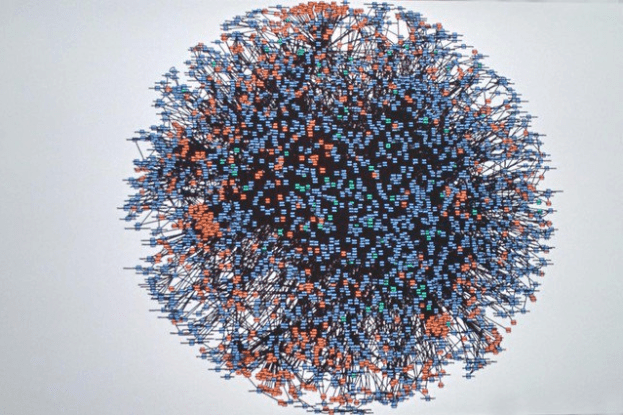
\includegraphics[scale = 0.5]{pictures/_kien_truc_vi_dich_vu_cua_amazon/main.png}

\caption{Kiến trúc vi dịch vụ của Amazon}

\end{figure}

% Đối với những doanh nghiệp không chuyển đổi kinh doanh sẽ không thể tồn tại.

% \begin{example} Gần đây, dịch vụ giao đồ ăn Baemin đã rời khỏi thị trường Việt Nam cũng do sức ép từ các đối thủ khác khiến Baemin khó cạnh tranh trong mảng kinh doanh cốt lõi là giao đồ ăn. Các đối thủ này không chỉ cung cấp dịch vụ giao đồ ăn mà còn có đặt xe, giao hàng, \dots

% \end{example}

% \begin{figure}[H]

% \centering

% 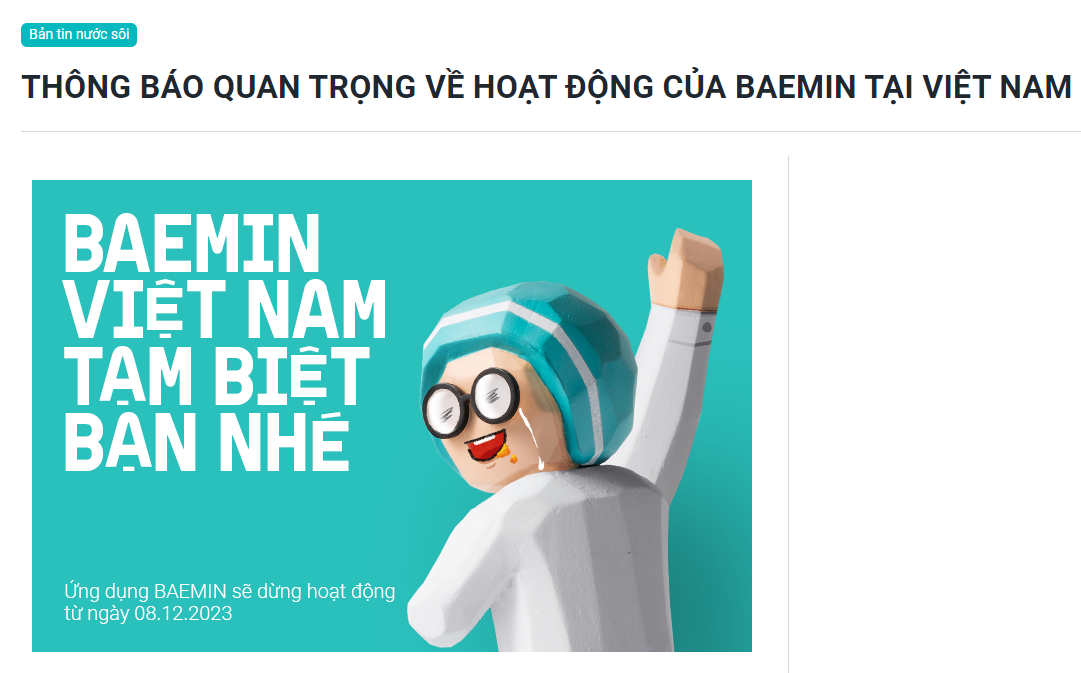
\includegraphics[scale = 0.5]{pictures/_baemin/main.png}

% \caption{Dịch vụ giao đồ ăn Baemin đã rời khỏi thị trường Việt Nam}

% \end{figure}

$\Rightarrow$ Hiện nay, các tổ chức doanh nghiệp có nhu cầu chuyển đổi kinh doanh để có thể tồn tại và phát triển khi thị trường thay đổi. Từ đó, đáp ứng nhu cầu của khách hàng, mang lại ưu thế cạnh tranh so với các đối thủ. Do đó, các doanh nghiệp cần hệ thống chuyển đổi nhanh chóng để đáp ứng nhu cầu của mô hình kinh doanh, đặt ra thách thức đối với kiến trúc phần mềm.



Kiến trúc nguyên khối đã phục vụ hiệu quả trong quá khứ, nhưng kiến trúc này bắt đầu gặp khó khăn khi đối mặt với sự phức tạp, khả năng mở rộng và khả năng đáp ứng linh hoạt. Kiến trúc vi dịch vụ là giải pháp cho những thách thức trên. Kiến trúc vi dịch vụ chia dự án thành những dịch vụ nhỏ độc lập, mỗi dịch vụ chịu trách nhiệm về một chức năng cụ thể tăng tính linh hoạt và chuyển đổi nhanh chóng.

% \section{Kiến trúc nguyên khối (Monolithic architecture)}
% Trước khi kiến trúc vi dịch vụ trở nên phổ biến, kiến trúc nguyên khối đã được áp dụng rộng rãi trong kiến trúc phần mềm truyền thống. \emph{Kiến trúc nguyên khối (Monolithic architecture)} là kiến trúc phần mềm trong đó tất cả các thành phần của dự án được xây dựng thành một đơn vị triển khai duy nhất.

Trong kiến trúc nguyên khối, bất kỳ thay đổi nào đối với một thành phần đều yêu cầu toàn bộ dự án phải được kiểm thử và triển khai lại dẫn đến tốc độ phát triển chậm và thiếu khả năng mở rộng.

Ví dụ: Mô hình MVC (Model - View - Controller) là một trong những mô hình phổ biến của kiến trúc nguyên khối. Trong mô hình này, ứng dụng được chia thành ba thành phần chính:

\begin{itemize}

\item \textbf{Mô hình (Model):} Đại diện cho dữ liệu và logic xử lý dữ liệu.

\item \textbf{Giao diện (View):} Đại diện cho giao diện người dùng.

\item \textbf{Bộ điều khiển (Controller):} Nhận yêu cầu người dùng thông qua giao diện, sau đó tương tác làm việc với dữ liệu.

\end{itemize}
% \section{Kiến trúc vi dịch vụ (Microservices architecture)}
% \emph{Kiến trúc vi dịch vụ (Microservices architecture)} chia dự án thành các thành phần nhỏ hơn được gọi là các dịch vụ.

\begin{itemize}

\item Mỗi dịch vụ tập trung vào một khả năng kinh doanh cụ thể.

\item Các dịch vụ độc lập và giao tiếp với nhau thông qua hạ tầng mạng.

\item Trong thực tế, nhiều dự án thường chuyển đổi một cách dần dần từ kiến trúc nguyên khối sang kiến trúc vi dịch vụ.

\end{itemize}

\begin{figure}[H]

\centering

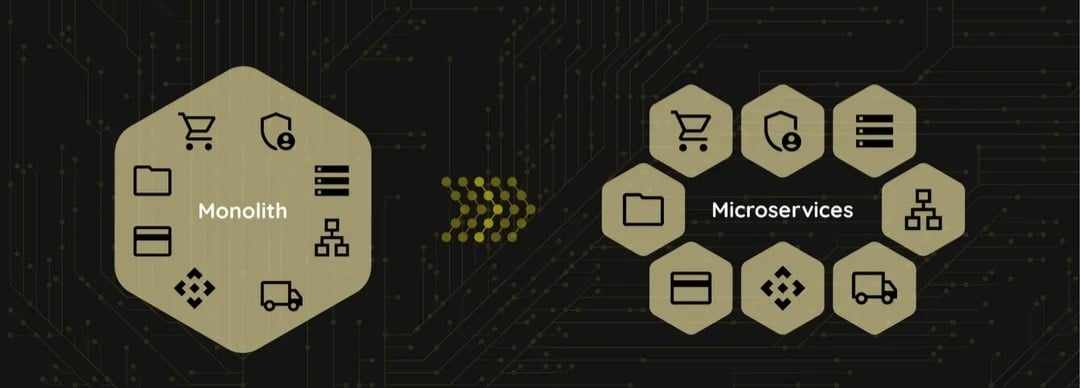
\includegraphics[scale = 0.4]{pictures/_chuyen_doi_tu_kien_truc_nguyen_khoi_sang_kien_truc_vi_dich_vu/main.drawio.png}

\caption{Chuyển đổi từ kiến trúc nguyên khối sang kiến trúc vi dịch vụ}

\end{figure}
% \section{Một số đặc điểm và ưu điểm của kiến trúc vi dịch vụ}
% Kiến trúc vi dịch vụ có nhiều ưu điểm, đặc biệt với các dự án có quy mô lớn và phức tạp.

\begin{itemize}

\item Kiến trúc vi dịch vụ phân chia dự án thành các dịch vụ nhỏ.

\begin{itemize}

\item Giúp việc phát triển và quản lý hệ thống dễ dàng hơn.

\item Tận dụng tài nguyên theo nhu cầu cho từng dịch vụ riêng.

\end{itemize}

\item Các dịch vụ độc lập về nghiệp vụ kinh doanh.

Các nhóm không cần hiểu sâu về mọi khía cạnh kinh doanh. Dẫn tới tốc độ phát triển và tốc độ định giá doanh nghiệp nhanh hơn.

\item Các dịch vụ độc lập về ngôn ngữ lập trình và CSDL

\begin{example} Mỗi dịch vụ sử dụng ngôn ngữ lập trình và CSDL khác nhau như: NodeJS, Go, Python, Java, CSharp, MongoDB, SQLServer, SQLite, MySQL, PostgreSQL, \dots

\end{example}

\begin{figure}[H]

\centering

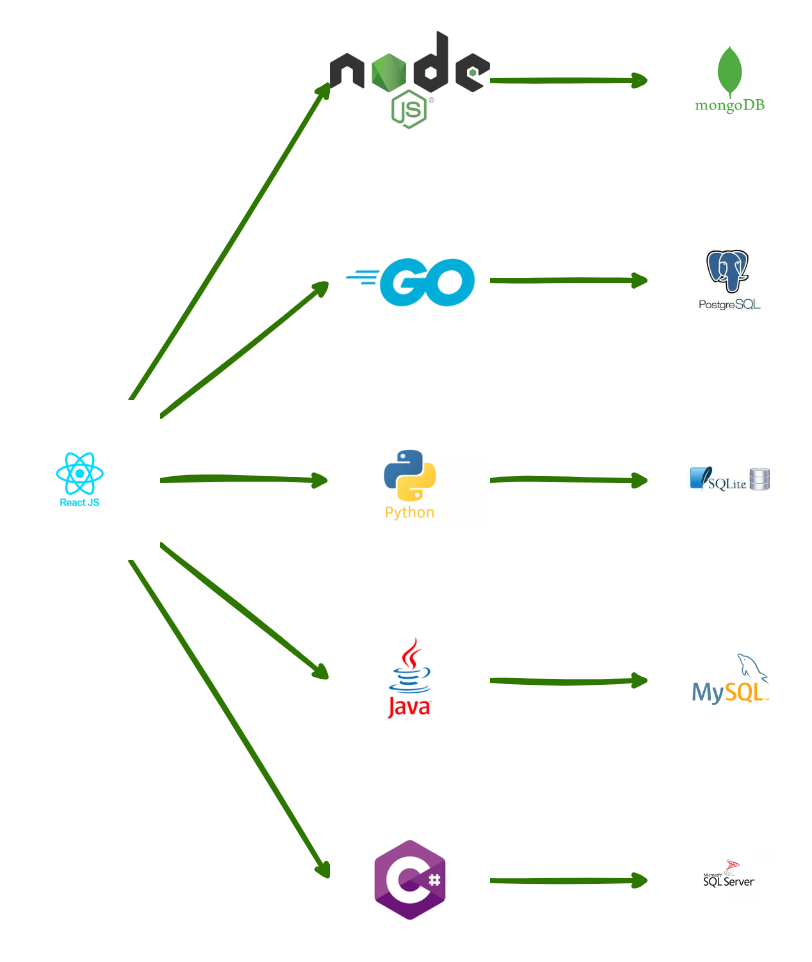
\includegraphics[scale = 0.3]{pictures/_da_ngon_ngu_va_csdl/main.drawio.png}

\caption{Các dịch vụ độc lập về ngôn ngữ lập trình và CSDL}

\end{figure}

\begin{itemize}

\item Kiến trúc vi dịch vụ sử dụng đa ngôn ngữ và công nghệ khác nhau. Từ đó tận dụng hiệu quả thế mạnh của từng ngôn ngữ, công nghệ phù hợp nhất cho yêu cầu nghiệp vụ cụ thể.

\end{itemize}

\item Các dịch vụ độc lập về triển khai hệ thống

Mỗi dịch vụ triển khai độc lập và có thể thay đổi mà không ảnh hưởng đến các dịch vụ khác.

Giảm ràng buộc và tăng tính linh hoạt của hệ thống. Từ đó dễ dàng mở rộng hệ thống.

\item Hệ thống có khả năng chịu lỗi tăng độ tin cậy.

Do các dịch vụ độc lập, nhiều dịch vụ có thể triển khai trong cùng một khả năng kinh doanh để đảm bảo tính sẵn sàng của hệ thống.

\end{itemize}
% \section{Một số nhược điểm và thách thức của kiến trúc vi dịch vụ}
% Mặc dù kiến trúc vi dịch vụ có nhiều lợi ích, nhưng cũng có nhiều thách thức:

\begin{itemize}

\item Chịu ảnh hưởng của đường truyền mạng.

\item Đồng bộ đồng hồ thời gian.

\item Ràng buộc về thứ tự sự kiện.

\item Tính nhất quán và toàn vẹn của dữ liệu.

\item Khả năng kiểm soát giao dịch.

\item Giám sát giữa các dịch vụ.

\item Bảo mật giao tiếp giữa các dịch vụ.

\item Phát hiện lỗi và sửa lỗi khó khăn, phức tạp hơn.

\item Chi phí xây dựng và quản lý vận hành lớn.

\end{itemize}
\chapter{Tìm hiểu về thiết kế hướng miền}

% Kiến trúc vi dịch vụ hỗ trợ doanh nghiệp chuyển đổi kinh doanh nhanh và mở rộng hệ thống dễ dàng. Tuy nhiên, để xây dựng được một kiến trúc vi dịch vụ tốt, cần phải tạo ra các dịch vụ nhỏ phù hợp và duy trì tính độc lập. Trong đồ án này, em sử dụng thiết kế hướng miền để phân tích và xây dựng kiến trúc vi dịch vụ. Thiết kế hướng miền giúp xác định và tổ chức các dịch vụ dựa trên việc hiểu rõ về lĩnh vực kinh doanh, từ đó giúp dự án phản ánh đúng các quy trình kinh doanh.
% \section{Đôi nét về thiết kế hướng miền (Domain Driven Design)}
% Thiết kế hướng miền được \emph{Eric Evans} giới thiệu trong cuốn sách \emph{"Domain Driven Design: Tackling Complexity in the Heart of Software"}. \emph{Thiết kế hướng miền (Domain Driven Design)} là một hướng tiếp cận thiết kế phần mềm tập trung vào việc hiểu rõ và mô hình hóa lĩnh vực kinh doanh của một tổ chức. Thiết kế hướng miền nhấn mạnh việc sử dụng lĩnh vực nghiệp vụ kinh doanh để thảo luận và đề xuất giải pháp đáp ứng nhu cầu.

Với nhiều phần mềm được thiết kế không tốt, phần xử lý các công việc không liên quan đến vấn đề nghiệp vụ kinh doanh như truy cập tập tin, hạ tầng mạng, cơ sở dữ liệu, \dots được lập trình trong đối tượng nghiệp vụ kinh doanh. Cách này có ưu điểm giúp tốc độ hoàn thiện phần mềm nhanh. Tuy nhiên, cách này làm dự án bị mất đi tính hướng đối tượng khó thay đổi, mở rộng hệ thống, \dots Thiết kế hướng miền cung cấp một cách để tổ chức mã nguồn và dễ dàng thích ứng với các yêu cầu thay đổi.
















% \subsection{Định nghĩa về miền (Domain)}
% Hệ thống phần mềm được tạo ra để xử lý công việc trong cuộc sống hiện đại. Việc phát triển hệ thống liên kết chặt chẽ với một số khía cạnh cụ thể trong cuộc sống của chúng ta. Trong thiết kế hướng miền, \emph{miền (Domain)} đề cập đến phạm vi kiến thức và vấn đề cụ thể mà hệ thống xử lý.

\begin{itemize}

\item Về góc độ kinh doanh: Miền đại diện cho một lĩnh vực hoặc ngành mà doanh nghiệp hoạt động.

\item Về góc độ hệ thống: Miền có thể coi là đại diện cho không gian vấn đề của hệ thống.

\end{itemize}

\begin{example} Trong đồ án này, miền được xác định là bài toán giải pháp hóa đơn điện tử. \end{example}
% \subsection{Chuyên gia miền (Domain Expert)}
% Trong thiết kế hướng miền, \emph{chuyên gia miền (Domain Expert)} là người có kiến thức và hiểu biết sâu sắc về vấn đề đang được hệ thống phần mềm giải quyết. Chuyên gia miền thể hiện chính xác vấn đề kinh doanh, đóng vai trò là nguồn thông tin cho nhóm phát triển.

Trong kiến trúc vi dịch vụ, thiết kế hướng miền đảm bảo mỗi dịch vụ được thiết kế phản ánh một phần cụ thể của lĩnh vực kinh doanh. Mỗi dịch vụ được quản lí bởi một nhóm phát triển được hỗ trợ bởi các chuyên gia miền.
% \subsection{Mô hình miền (Domain Models)}
% Để tạo một phần mềm tốt, chúng ta cần phải hiểu rõ về phần mềm đó. \emph{Mô hình miền (Domain Models)} là kiến thức có tổ chức và có cấu trúc về miền phù hợp để giải quyết vấn đề kinh doanh. Mục tiêu của mô hình miền là cung cấp rõ ràng, ngắn gọn và chính xác về miền làm cơ sở để hệ thống giải quyết vấn đề kinh doanh.

\begin{example} Trong đồ án này, mô hình miền của em là các sơ đồ mẫu kỹ thuật ở phần \emph{"Các mẫu kỹ thuật trong thiết kế hướng miền"}. \end{example}
% \subsection{Cốt lõi của thiết kế hướng miền}
% Thiết kế hướng miền cung cấp 2 loại mẫu:

\begin{itemize}

\item \emph{Các mẫu chiến lược (Strategic Patterns):} Phân chia một miền lớn và phức tạp thành các phần nhỏ hơn với ranh giới được xác định rõ ràng. Giúp phân chia một miền lớn hợp lý.

\item \emph{Các mẫu kỹ thuật (Tactical Patterns):} Hiện thực hóa các khái niệm và qui trình thành các thiết kế hệ thống phần mềm. Giúp hệ thống phù hợp với kinh doanh.

\end{itemize}

\begin{figure}[H]

\centering

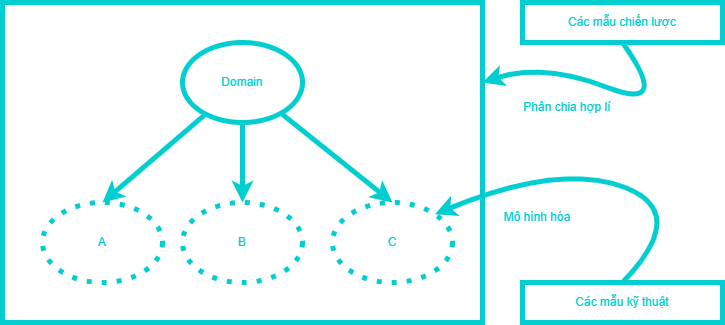
\includegraphics[scale = 0.5]{pictures/_tong_quan_ve_cot_loi_cua_thiet_ke_huong_mien/main.drawio.png}

\caption{Tổng quan về cốt lõi của thiết kế hướng miền}

\end{figure}

% \newpage
% \section{Các mẫu chiến lược trong thiết kế hướng miền}
% Các mẫu chiến lược giúp xác định các thành phần quan trọng của hệ thống. Các mẫu chiến lược phân tích nghiệp vụ kinh doanh sau đó đưa ra việc phân chia các thành phần và hiểu mối quan hệ của các thành phần đó. Từ việc phân chia hệ thống thành các thành phần nhỏ, chúng ta có thể tạo ra hệ thống mở rộng dễ dàng, phát triển linh hoạt theo nhu cầu kinh doanh.

Các mẫu chiến lược bao gồm:

\begin{itemize}

\item Miền phụ (Sub - Domain)

% !trình bày thêm nội dung nhỏ

% !trình bày thêm nội dung nhỏ

% !trình bày thêm nội dung nhỏ

% !trình bày thêm nội dung nhỏ

% !trình bày thêm nội dung nhỏ

% !trình bày thêm nội dung nhỏ

% !trình bày thêm nội dung nhỏ

% !trình bày thêm nội dung nhỏ

% !trình bày thêm nội dung nhỏ

% !trình bày thêm nội dung nhỏ

% !trình bày thêm nội dung nhỏ

% !trình bày thêm nội dung nhỏ

\item Miền phụ (Sub - Domain)

\item Miền phụ (Sub - Domain)

\item Miền phụ (Sub - Domain)

\item Miền phụ (Sub - Domain)

\item Miền phụ (Sub - Domain)

\item Miền phụ (Sub - Domain)

\end{itemize}

\begin{figure}[H]

\centering

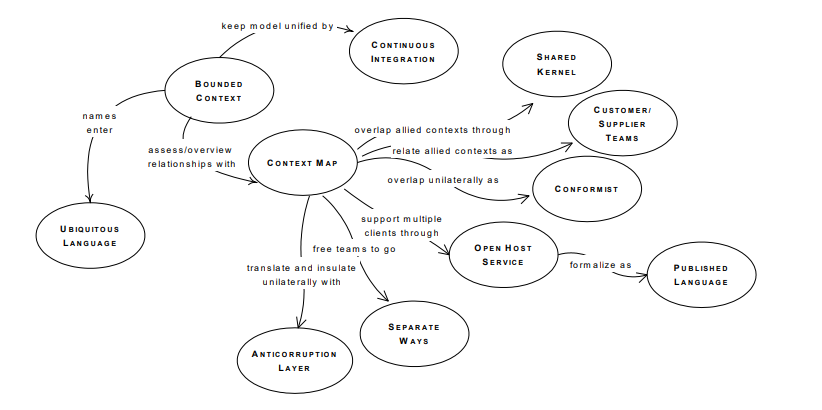
\includegraphics[scale = 0.9]{pictures/cac_mau_chien_luoc/temp.png}

\caption{Sơ đồ về các thành phần trong mẫu chiến lược}

\end{figure}

% !<! - - $ Vẽ lại sau khi trình bày xong các mục nhỏ - - >
% \subsection{Miền phụ (Sub - Domain)}
% Một miền kinh doanh lớn được tạo thành từ nhiều \emph{miền phụ (Sub - Domain)}. Trong thực tế, một miền kinh doanh phức tạp không thể có một chuyên gia miền có kiến thức về tất cả các miền phụ.

\begin{example} Trong miền thương mại điện tử lớn có thể có một số miền phụ sau:

\begin{itemize}

\item \textbf{Miền phụ quản lý hàng tồn kho:} liên quan đến việc quản lý sản phẩm trong kho hàng.

\item \textbf{Miền phụ quản lý khách hàng:} liên quan đến việc quản lý tài khoản khách hàng.

\item \textbf{Miền phụ vận chuyển:} liên quan đến việc quản lý việc vận chuyển giao hàng.

\end{itemize}

\end{example}

\subsubsection{Phân loại các miền phụ}

Trong thiết kế hướng miền, có ba loại miền phụ là:

\begin{itemize}

\item Miền phụ chung (Generic Subdomain)

Miền phụ chung cung cấp các giải pháp có sẵn mà doanh nghiệp có thể mua. Miền phụ chung có thể được tìm thấy trên nhiều ngành. Doanh nghiệp không thể đạt được bất kỳ lợi thế cạnh tranh so với đối thủ bằng cách thực hiện những điều khác biệt trong miền phụ chung.

\begin{example} Các miền phụ chung \emph{"quản lý nhân sự"} hay \emph{"quản lý cơ sở vật chất"} không tạo thêm bất kỳ giá trị khác biệt nào cho doanh nghiệp. \end{example}

\item Miền phụ cốt lõi (Core Subdomain)

Miền phụ cốt lõi là phần quan trọng và có giá trị nhất của hệ thống. Miền phụ cốt lõi giúp phân biệt các doanh nghiệp và làm cho các doanh nghiệp có giá trị. Miền phụ cốt lõi tập trung vào mục tiêu và yêu cầu của khách hàng với doanh nghiệp, từ đó quyết định sự thành công của doanh nghiệp. Vì vậy, mỗi doanh nghiệp luôn tìm cách thực hiện những điều khác biệt trong các miền phụ cốt lõi này để đạt được lợi thế so với đối thủ cạnh tranh.

\begin{example} Trong miền thẻ tín dụng, miền phụ cốt lõi có thể là \emph{"phát hành thẻ"} chịu trách nhiệm về quá trình phát hành thẻ tín dụng cho khách hàng. Miền phụ cốt lõi này bao gồm các nhiệm vụ như: thu thập thông tin khách hàng, thực hiện kiểm tra tín dụng, kích hoạt thẻ, \dots \end{example}

\item Miền phụ hỗ trợ (Supporting Subdomain)

Các miền phụ cốt lõi phụ thuộc vào các miền phụ hỗ trợ. Miền phụ hỗ trợ cung cấp các dịch vụ để miền phụ cốt lõi hoạt động hiệu quả. Tuy nhiên, miền phụ hỗ trợ không đòi hỏi mức độ phức tạp cao về logic nghiệp vụ.

\begin{example} Trong nhiều phần mềm, miền phụ hỗ trợ \emph{"xác thực người dùng"} OAuth 2.0 của Facebook hoặc Google hỗ trợ cho miền phụ cốt lõi hoạt động. \end{example}

\end{itemize}

\subsubsection{Cách xác định miền phụ}

Các miền phụ cốt lõi, hỗ trợ và chung có thể khác nhau đối với các doanh nghiệp vì tùy theo nhu cầu kinh doanh và bối cảnh cụ thể của mỗi tổ chức.

\textbf{Các bước xác định miền phụ:}

\begin{enumerate}

\item Bắt đầu bằng cách xem xét nghiệp vụ kinh doanh.

\item Nếu có sẵn giải pháp đã biết thì có khả năng là miền phụ chung. Ngược lại, chúng ta kiểm tra xem nghiệp vụ kinh doanh đó có thêm giá trị kinh doanh nào hay không?

\item Nếu không có giá trị kinh doanh thì chúng ta kiểm tra xem các miền phụ cốt lõi có phụ thuộc vào miền phụ này hay không? Nếu có thì có khả năng là miền phụ hỗ trợ. Nếu không thì đó là miền phụ chung.

\item Nếu miền phụ có tiềm năng bổ sung một số giá trị kinh doanh thì bước kiểm tra tiếp theo là xem liệu miền doanh nghiệp có độ phức tạp cao hay không?

\item Nếu miền doanh nghiệp không có độ phức tạp cao thì có khả năng là miền phụ hỗ trợ. Ngược lại thì nó có khả năng là miền phụ cốt lõi.

\end{enumerate}

\begin{figure}[H]

\centering

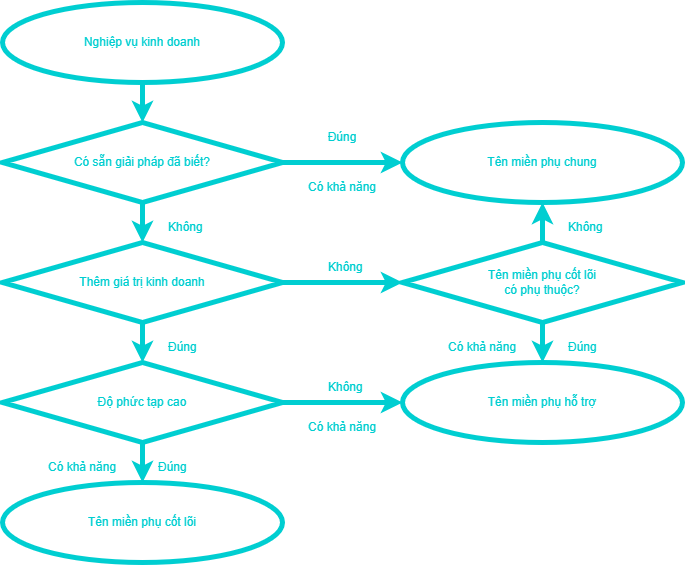
\includegraphics[scale = 0.5]{pictures/_so_do_xac_dinh_mien_phu/main.drawio.png}

\caption{Sơ đồ xác định miền phụ}

\end{figure}

\subsubsection{Áp dụng phân loại miền phụ trong đồ án này}

\begin{itemize}

\item Từ yêu cầu nghiệp vụ, em có thể phân chia thành các miền phụ như sau:

\begin{itemize}

\item Quản lý hóa đơn

\item Báo cáo thống kê

\item Thông báo

\item Thư điện tử

\item Quản lý hệ thống

\end{itemize}

\item Phân loại miền phụ

\begin{itemize}

\item Miền phụ chung

Có thể là các miền có sẵn, hoạt động ổn định, không được đề cập trong nghiệp vụ phần mềm hóa đơn điện tử như:

\begin{itemize}

\item Quản lý nhân sự

\item Quản lý cơ sở vật chất

\end{itemize}

\item Miền phụ cốt lõi

\begin{itemize}

\item Quản lý hóa đơn

Là miền cốt lõi quan trọng tạo lợi thế cạnh tranh trong ngành.

\item Báo cáo thống kê

Giúp theo dõi tình hình thông tin tài chính của doanh nghiệp.

\item Thông báo

Miền thông báo giúp hỗ trợ thông tin các quy định về thuế và pháp luật đến với khách hàng sử dụng.

\item Quản lý hệ thống

Miền này giúp xác thực và ủy quyền bảo vệ dữ liệu của khách hàng.

\end{itemize}

\item Miền phụ hỗ trợ

\item \begin{itemize}

\item Thư điện tử

Miền thư điện tử hỗ trợ miền cốt lõi trao đổi thông tin với khách hàng.

\end{itemize}

\end{itemize}

\end{itemize}
% \subsection{Ngôn ngữ chung (Ubiquitous Language)}
% Trong quá trình xây dựng hệ thống, cần có trao đổi giữa người thiết kế hệ thống và chuyên gia miền. Tuy nhiên, nhóm kinh doanh sử dụng ngôn ngữ kinh doanh và nhóm công nghệ có xu hướng sử dụng các thuật ngữ kỹ thuật trong giao tiếp của họ. Người phát triển phần mềm tập trung vào lớp, phương thức, thuật toán, \dots Chuyên gia miền thường sử dụng ngôn ngữ chuyên ngành của họ. Sự khác biệt về ngôn ngữ giữa các thành viên có thể dẫn đến những thách thức về giao tiếp. Ngoài ra, trong các lĩnh vực kinh doanh khác nhau, một thuật ngữ có thể được sử dụng trong nhiều miền, cùng với ý nghĩa khác nhau gây ra sự nhầm lẫn và hiểu sai cho các người phát triển phần mềm cũng như các chuyên gia miền.

Thiết kế hướng miền đề xuất sử dụng ngôn ngữ chung để giải quyết những thách thức ngôn ngữ. \emph{Ngôn ngữ chung (Ubiquitous Language)} là một ngôn ngữ được cấu trúc xung quanh mô hình miền và được tất cả các thành viên trong nhóm sử dụng cho mọi hoạt động của nhóm với phần mềm. Ngôn ngữ chung được xác định bởi các từ vựng và có định nghĩa rõ ràng về ngữ cảnh sử dụng từ vựng.

\subsubsection{Một số đặc điểm của ngôn ngữ chung}

\begin{itemize}

\item Ngôn ngữ chung được sử dụng bởi cả chuyên gia miền và chuyên gia công nghệ.

\item Có nhiều ngôn ngữ chung trong một tổ chức được mỗi nhóm tạo và quản lý độc lập.

\item Việc tạo ra ngôn ngữ chung là một quá trình liên tục, phát triển theo thời gian qua sự cộng tác giữa chuyên gia miền và chuyên gia công nghệ.

\item Các thành viên phải sử dụng ngôn ngữ chung cho các công việc và trong hệ thống.

\end{itemize}

\begin{figure}[H]

\centering

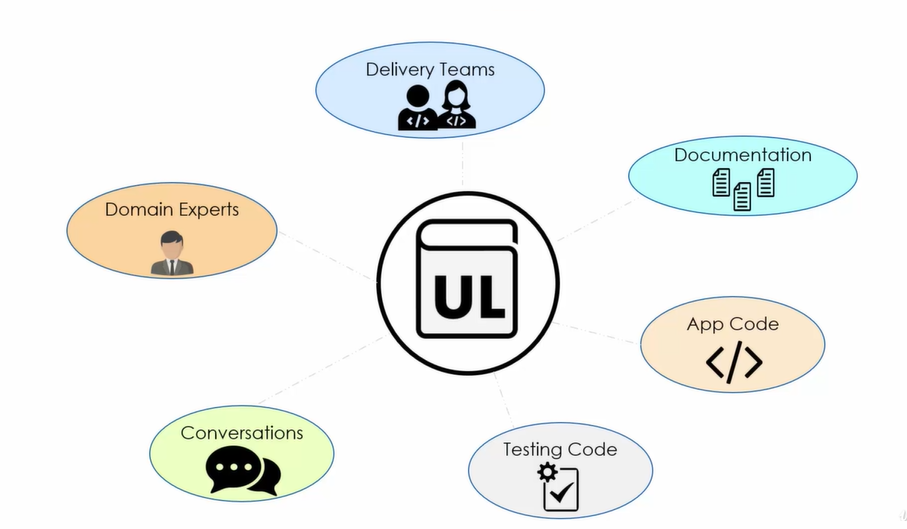
\includegraphics[scale = 0.6]{pictures/_ngon_ngu_chung_duoc_su_dung_trong_toan_bo_he_thong/main.png}

\caption{Ngôn ngữ chung được sử dụng trong toàn bộ hệ thống}

\end{figure}

\begin{example} Trong đồ án này, em đã sử dụng ngôn ngữ chung trong toàn bộ hệ thống của mình từ yêu cầu nghiệp vụ, mã nguồn, kiểm thử, \dots \end{example}
% \subsection{Tích hợp liên tục (Continuous Integration)}
% Khi phân chia miền lớn thành các miền phụ nhỏ hơn, chúng ta cần đảm bảo rằng các miền phụ luôn ở trạng thái mới và hoạt động tốt như kỳ vọng, hạn chế xảy ra xung đột. Đáp ứng nhu cầu doanh nghiệp phát triển thay đổi liên tục và nhanh chóng.

\emph{Tích hợp liên tục (Continuous Integration)} là công nghệ tích hợp mã nguồn liên tục, tự động kiểm thử giúp phát hiện và sửa lỗi sớm hơn, giảm thời gian cũng như rủi ro trong quá trình phát triển.







% \begin{example} Jenkins là một công cụ tiêu biểu trong công nghệ tích hợp liên tục. \end{example}

% \begin{figure}[H]

% \centering

% 
\includegraphics[scale = 0.4]{pictures/_vi_du_ve_jenkins_trong_cong_nghe_tich_hop_lien_tuc/main.png}

% \caption{Ví dụ về Jenkins trong công nghệ tích hợp liên tục.}

% \end{figure}
% \subsection{Bối cảnh bị giới hạn (Bounded Context)}
% Một miền cần chia đủ nhỏ để phù hợp với một nhóm cụ thể. Để đạt được điều này, chúng ta cần xác định rõ ranh giới giữa các ngữ cảnh. \emph{Bối cảnh bị giới hạn (Bounded Context)} giúp xác định rõ các ranh giới, chia miền thành các phần độc lập để giải quyết sự phức tạp trong mô hình doanh nghiệp. Bối cảnh bị giới hạn tạo ra các mô hình khác nhau cho các lĩnh vực khác nhau của miền. Bối cảnh bị giới hạn thể hiện phạm vi kinh doanh của dịch vụ.

\begin{figure}[H]

    \centering

    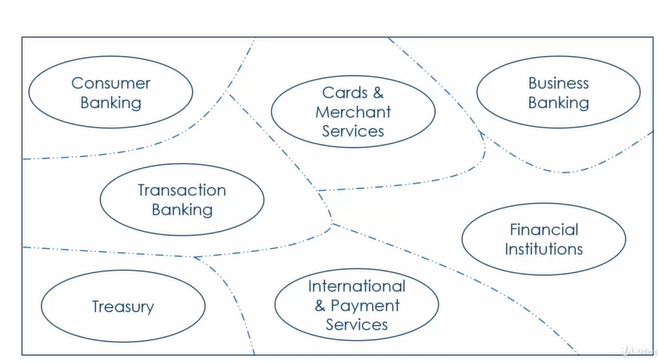
\includegraphics[scale = 1]{pictures/boi_canh_gioi_han/main.png}

    \caption{Ví dụ về bối cảnh bị giới hạn trong một ngân hàng}

\end{figure}

\subsubsection{Cách xác định bối cảnh bị giới hạn}

Để có thể xác định được bối cảnh bị giới hạn chúng ta có thể xem xét:

\begin{itemize}

    \item Dựa vào việc phân chia các miền phụ.

    \item Dựa vào sơ đồ cấu trúc tổ chức các phòng ban của doanh nghiệp.

    \item Dựa vào modules của các ứng dụng kiến trúc nguyên khối (nếu việc phân chia tốt).

    \item Dựa vào trách nhiệm và hoạt động của chuyên gia miền .

\end{itemize}

% \subsubsection{Áp dụng xác định bối cảnh bị giới hạn trong đồ án này}

% \subsubsection{Áp dụng xác định bối cảnh bị giới hạn trong đồ án này}

% \subsubsection{Áp dụng xác định bối cảnh bị giới hạn trong đồ án này}

% \subsubsection{Áp dụng xác định bối cảnh bị giới hạn trong đồ án này}

% \subsubsection{Áp dụng xác định bối cảnh bị giới hạn trong đồ án này}

% \subsubsection{Áp dụng xác định bối cảnh bị giới hạn trong đồ án này}

% \subsubsection{Áp dụng xác định bối cảnh bị giới hạn trong đồ án này}

% \subsubsection{Áp dụng xác định bối cảnh bị giới hạn trong đồ án này}

% \subsubsection{Áp dụng xác định bối cảnh bị giới hạn trong đồ án này}

% \subsubsection{Áp dụng xác định bối cảnh bị giới hạn trong đồ án này}

% \subsubsection{Áp dụng xác định bối cảnh bị giới hạn trong đồ án này}

% \subsubsection{Áp dụng xác định bối cảnh bị giới hạn trong đồ án này}

%!<! - - Hướng dẫn 5/10 - - >

%!<! - - Hướng dẫn 5/10 - - >

%!<! - - Hướng dẫn 5/10 - - >

%!<! - - Hướng dẫn 5/10 - - >

%!<! - - Hướng dẫn 5/10 - - >

%!<! - - Hướng dẫn 5/10 - - >

%!<! - - Hướng dẫn 5/10 - - >

%!<! - - Hướng dẫn 5/10 - - >

%!<! - - Hướng dẫn 5/10 - - >

% \subsection{Mối quan hệ bối cảnh bị giới hạn (Bounded Context Relationships)}
% Có 3 loại mối quan hệ giữa các bối cảnh bị giới hạn là:

\begin{itemize}

\item Mối quan hệ đối xứng (Symmetric Relationship)

\textbf{Mô tả:} Thể hiện sự tương tác 2 chiều giữa 2 bối cảnh bị giới hạn.

\item Mối quan hệ bất đối xứng (Asymmetric Relationship)

\textbf{Mô tả:} Thể hiện sự tương tác 1 chiều giữa 2 các bối cảnh bị giới hạn.

\item Mối quan hệ 1 - nhiều (One to Many Relationship)

\textbf{Mô tả:} Thể hiện sự tương tác 1 chiều giữa 1 bối cảnh bị giới hạn với nhiều bối cảnh bị giới hạn khác.

\end{itemize}

\begin{figure}[H]

\centering

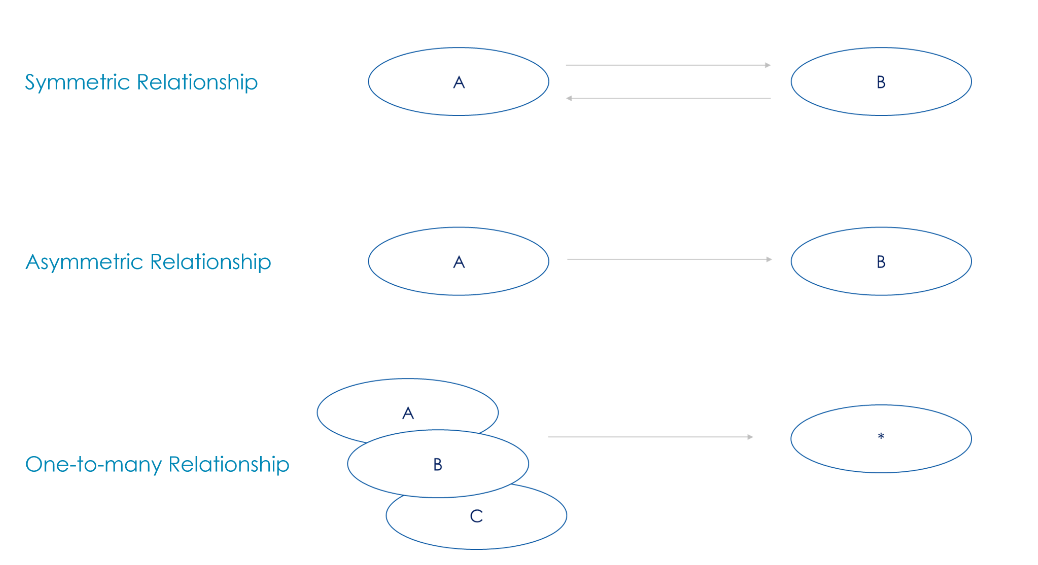
\includegraphics[scale = 0.5]{pictures/cac_moi_quan_he_boi_canh_gioi_han/main.png}

\caption{Các mối quan hệ bối cảnh bị giới hạn}

\end{figure}

\subsubsection{Mối quan hệ đối xứng (Symmetric Relationship)}

\paragraph{Mô hình riêng biệt (Separate Ways)}

Khi các bối cảnh bị giới hạn có quan hệ riêng biệt, không có sự phụ thuộc. Vì vậy, các bối cảnh bị giới hạn này có ngôn ngữ, mô hình, mục đích độc lập và thực thi riêng biệt. Các nhóm phát triển không phải cộng tác hay phối hợp với nhau từ đó đem lại lợi ích dễ dàng bảo trì và mở rộng hệ thống.

\begin{example} Trong miền ngân hàng, thẻ tín dụng và khoản vay mua nhà không có mối quan hệ.

\begin{figure}[H]

\centering

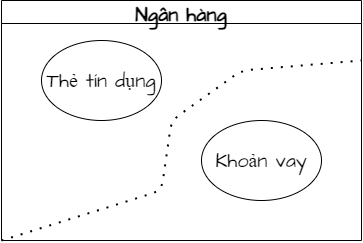
\includegraphics[scale = 0.5]{pictures/mo_hinh_rieng_biet_separate_ways/main.drawio.png}

\caption{Ví dụ mô hình riêng biệt (Separate Ways)}

\end{figure}

\end{example}

\paragraph{Mô hình hạt nhân chung (Shared Kernel)}

Trong thực tế, nhiều bối cảnh bị giới hạn phụ thuộc lẫn nhau. Mô hình hợp tác (Partnership) tạo điều kiện cho việc giao tiếp và cộng tác giữa các bối cảnh bị giới hạn phụ thuộc. Tuy nhiên, sự phụ thuộc này dẫn đến mức độ kết hợp cao giữa các nhóm và bối cảnh bị giới hạn, dẫn tới mất đi tính độc lập.

\emph{Lưu ý: Mô hình hợp tác không phải là mô hình của các mẫu chiến lược trong thiết kế huớng miền.}

Để giải quyết vấn đề bối cảnh bị giới hạn phụ thuộc lẫn nhau chúng ta có mô hình hạt nhân chung. Mô hình hạt nhân chung (Shared Kernel) cho phép các bối cảnh bị giới hạn có phần chia sẻ chung và có ranh giới phân định rõ ràng. Từ đó, tách việc quản lí các mô hình hạt nhân chung này một cách độc lập với phần còn lại của bối cảnh bị giới hạn. Khi cần thay đổi mà không phải của mô hình hạt nhân chung thì nhóm sẽ hoạt động độc lập. Thông thường, mô hình hạt nhân chung được hiện thực hóa bằng các thư viện chung. Tuy nhiên, chỉ sử dụng mô hình hạt nhân chung nếu quan hệ của các bối cảnh bị giới hạn nhỏ và ổn định để tránh quan hệ phức tạp và ràng buộc chặt chẽ.

\begin{example} Trong miền ngân hàng, thẻ tín dụng và khoản vay mua nhà không có mối quan hệ.

\begin{figure}[H]

\centering

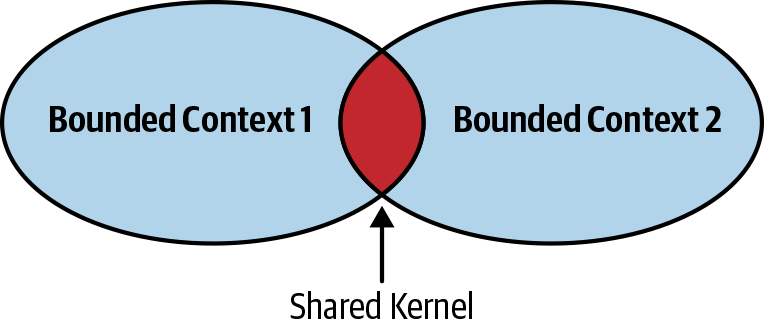
\includegraphics[scale = 1]{pictures/_vi_du_mo_hinh_hat_nhan_chung_shared_kernel/main.png}

\caption{Ví dụ mô hình hạt nhân chung (Shared Kernel)}

\end{figure}

\end{example}

\subsubsection{Mối quan hệ bất đối xứng (Asymmetric Relationship)}

Trong mối quan hệ bất đối xứng, một bối cảnh bị giới hạn có sự phụ thuộc vào một bối cảnh bị giới hạn khác. Mối quan hệ này được mô tả bằng cách gán vai trò cho bối cảnh bị giới hạn:

\begin{itemize}

\item \textbf{Bối cảnh bị giới hạn thượng nguồn (Upstream):}

\begin{itemize}

\item Bối cảnh bị giới hạn cung cấp cho bối cảnh bị giới hạn khác. Ký hiệu: U

\end{itemize}

\item \textbf{Bối cảnh bị giới hạn hạ lưu (Downstream):}

\begin{itemize}

\item Bối cảnh bị giới hạn phụ thuộc vào bối cảnh bị giới hạn khác. Ký hiệu: D

\end{itemize}

\end{itemize}

\begin{example} Mối quan hệ bất đối xứng giữa bối cảnh bị giới hạn A và bối cảnh bị giới hạn B.

\begin{itemize}

\item Bối cảnh bị giới hạn A ràng buộc với bối cảnh bị giới hạn B

\item Bối cảnh bị giới hạn A đóng vai trò là bối cảnh bị giới hạn hạ lưu (Downstream)

\item Bối cảnh bị giới hạn B đóng vai trò là bối cảnh bị giới hạn thượng nguồn (Upstream)

\item Bối cảnh bị giới hạn A có kiến thức về các mô hình trong bối cảnh bị giới hạn B

\item Bối cảnh bị giới hạn B không có bất kỳ kiến thức nào về mô hình trong bối cảnh bị giới hạn A

\end{itemize}

\begin{figure}[H]

\centering

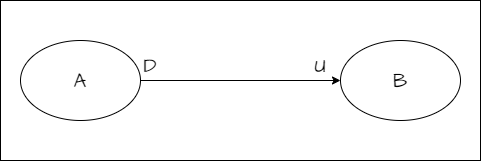
\includegraphics[scale = 0.5]{pictures/moi_quan_he_bat_doi_xung/main.drawio.png}

\caption{Ví dụ mối quan hệ bất đối xứng}

\end{figure}

\end{example}

\paragraph{Mô hình khách hàng - nhà cung cấp (Customer - Supplier)}

Được thể hiện rằng bối cảnh bị giới hạn thượng nguồn đáp ứng nhu cầu của bối cảnh bị giới hạn hạ lưu.

Khi đó:

\begin{itemize}

\item Bối cảnh bị giới hạn thượng nguồn được gọi là nhà cung cấp.

\item Bối cảnh bị giới hạn hạ lưu được gọi là khách hàng.

\end{itemize}

Trong thực tế, nhóm phát triển nhà cung cấp luôn tham khảo ý kiến của nhóm phát triển khách hàng và có bộ kiểm thử để đảm bảo rằng dịch vụ của nhà cung cấp đáp ứng được yêu cầu của khách hàng.

\paragraph{Mô hình tuân thủ (Conformist)}

Trong mô hình khách hàng - nhà cung cấp, nếu nhà cung cấp thực hiện tốt yêu cầu thì khách hàng cần tuân thủ chặt chẽ. Mô hình tuân thủ (Conformist) là một mối quan hệ trong đó bối cảnh bị giới hạn hạ lưu áp dụng mô hình, ngôn ngữ chung và các khái niệm của bối cảnh bị giới hạn thượng nguồn.

Trong mô hình tuân thủ bối cảnh bị giới hạn hạ lưu được ký hiệu là CF.

\begin{figure}[H]

\centering

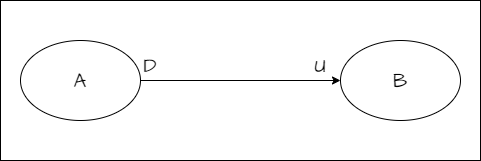
\includegraphics[scale = 0.5]{pictures/_vi_du_mo_hinh_tuan_thu_conformist/map.drawio.png}

\caption{Ví dụ mô hình tuân thủ (Conformist)}

\end{figure}

\paragraph{Mô hình chống đổ vỡ (Anti Corruption Layer)}

Trong mô hình khách hàng - nhà cung cấp, nếu nhà cung cấp có thể thay đổi linh hoạt không đảm bảo đáp ứng nhu cầu của khách hàng thì khách hàng cần có giải pháp xử lí. Mô hình chống đổ vỡ (Anti Corruption Layer) là một mối quan hệ trong đó bối cảnh bị giới hạn hạ lưu sử dụng một lớp để dịch giữa ngôn ngữ của nó và ngôn ngữ của bối cảnh bị giới hạn thượng nguồn.

Trong mô hình chống đổ vỡ, mỗi bối cảnh bị giới hạn có mô hình riêng biệt và lớp chống đổ vỡ cần kiến thức về mô hình hạ lưu và thượng nguồn để bảo vệ hạ lưu và duy trì tính toàn vẹn.

Trong mô hình chống đổ vỡ bối cảnh bị giới hạn hạ lưu được ký hiệu là ACL.

Mô hình chống đổ vỡ được hiện thực hóa bằng mẫu bộ điều hợp (Adapter pattern).

\begin{figure}[H]

\centering

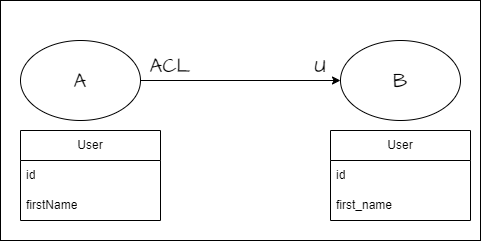
\includegraphics[scale = 0.5]{pictures/_vi_du_mo_hinh_chong_do_vo_anti_corruption_layer/map.drawio.png}

\caption{Ví dụ mô hình chống đổ vỡ (Anti Corruption Layer)}

\end{figure}

\subsubsection{Mối quan hệ 1 - nhiều (One to Many Relationship)}

\paragraph{Dịch vụ máy chủ mở (Open Host Service)}

Dịch vụ máy chủ mở (Open Host Service) là nhà cung cấp trong mô hình khách hàng - nhà cung cấp, dịch vụ máy chủ mở hiển thị một API công khai cho các bối cảnh bị giới hạn khác sử dụng chức năng của nhà cung cấp.

Trong bản đồ bối cảnh, dịch vụ máy chủ mở được ký hiệu là OHS.

\begin{figure}[H]

\centering

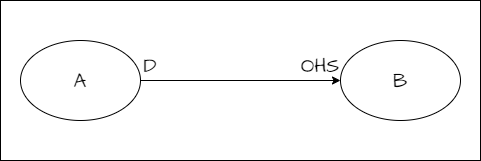
\includegraphics[scale = 0.5]{pictures/_vi_du_dich_vu_may_chu_mo_open_host_service/map.drawio.png}

\caption{Ví dụ dịch vụ máy chủ mở (Open Host Service)}

\end{figure}

\paragraph{Ngôn ngữ được xuất bản (Published Language)}

Khi ngôn ngữ chung ở dịch vụ máy chủ mở được các nhóm phát triển trong bối cảnh bị giới hạn hạ lưu chấp nhận. Ngôn ngữ chung này được gọi là ngôn ngữ được xuất bản (Published Language). Ngôn ngữ được xuất bản có lợi ích là tính thống nhất trong hệ thống tuy nhiên cần phân tích kĩ vì nó có thể tạo ra sự nhầm lẫn trong bối cảnh bị giới hạn hạ lưu nào đó.

Trong bản đồ bối cảnh, ngôn ngữ được xuất bản kết hợp dịch vụ máy chủ mở được ký hiệu là OHS|PL.

\begin{figure}[H]

\centering

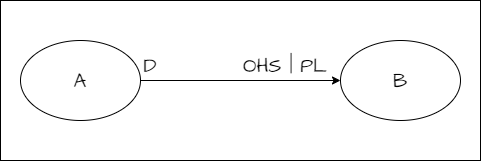
\includegraphics[scale = 0.5]{pictures/_vi_du_ngon_ngu_duoc_xuat_ban_published_language/map.drawio.png}

\caption{Ví dụ ngôn ngữ được xuất bản (Published Language)}

\end{figure}

% %%%%%%%%%%%%%%%%%%%%%%%%%%%%%%%%%%

% %%%%%%%%%%%%%%%%%%%%%%%%%%%%%%%%%%

% %%%%%%%%%%%%%%%%%%%%%%%%%%%%%%%%%%

% %%%%%%%%%%%%%%%%%%%%%%%%%%%%%%%%%%

% %%%%%%%%%%%%%%%%%%%%%%%%%%%%%%%%%%

% %%%%%%%%%%%%%%%%%%%%%%%%%%%%%%%%%%

% %%%%%%%%%%%%%%%%%%%%%%%%%%%%%%%%%%

% %%%%%%%%%%%%%%%%%%%%%%%%%%%%%%%%%%

% %! Hướng dẫn 6/6
% \subsection{Bản đồ bối cảnh (Context Maps)}
% Những mối quan hệ của bối cảnh bị giới hạn cần được quản lý chặt chẽ để hoạt động độc lập, nhất quán và linh hoạt. Do đó, chúng ta cần phải ghi lại các mối quan hệ thông qua việc sử dụng bản đồ bối cảnh. \emph{Bản đồ bối cảnh (Context Maps)} là sự thể hiện trực quan của hệ thống, thể hiện các thành phần và mối quan hệ giữa các thành phần.

\begin{figure}[H]

    \centering

    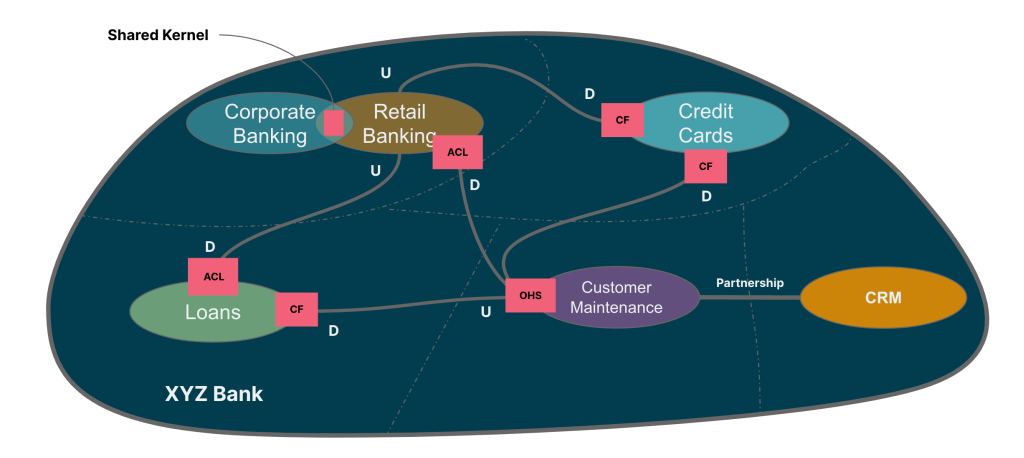
\includegraphics[scale = 0.4]{pictures/_vi_du_ban_do_boi_canh_trong_1_ngan_hang/main.drawio.png}

    \caption{Ví dụ bản đồ bối cảnh trong 1 ngân hàng}

\end{figure}


\subsubsection{Áp dụng bản đồ bối cảnh}
% Do sử dụng adapter\dots

%@# \chapter{Phân tích thiết kế hệ thống}
%@# \section{UML Use Case Diagrams}
%@# \section{UML Activity Diagrams}
%@# \section{UML Sequence Diagrams}
%@# \section{UML Class Diagrams}

% \newpage
\section{Các mẫu kỹ thuật trong thiết kế hướng miền}
% Các mẫu kỹ thuật được sử dụng để lập mô hình và hiện thực hóa các thành phần riêng lẻ của hệ thống dịch vụ vi mô. Các mẫu kỹ thuật tập trung mô hình hóa miền và triển khai logic nghiệp vụ trong lập trình.

\begin{figure}[H]

\centering

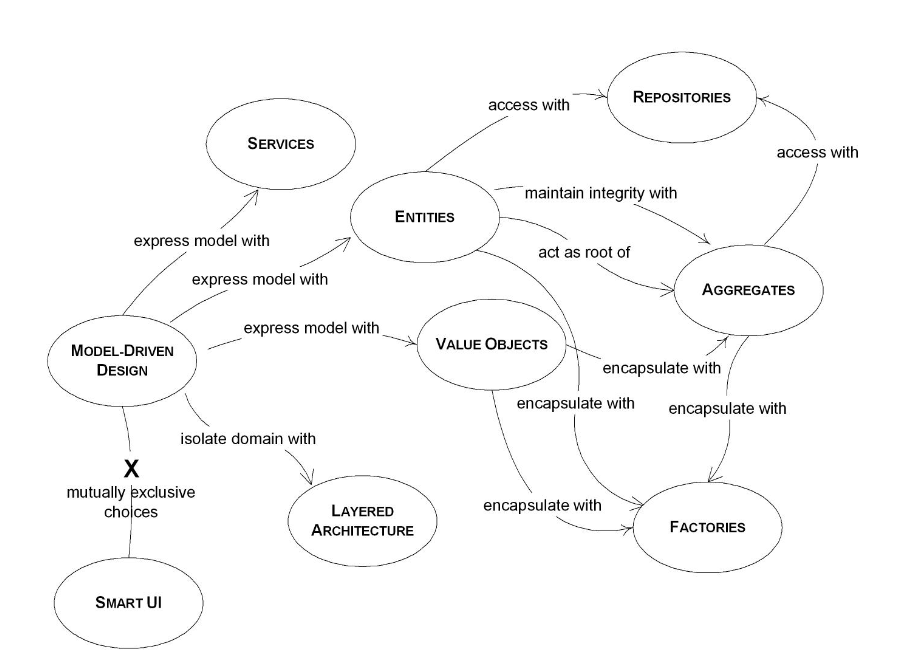
\includegraphics[scale = 0.5]{pictures/cac_mau_ky_thuat/temp.png}

\caption{Sơ đồ về các thành phần trong mẫu kỹ thuật}

\end{figure}
\subsection{Đối tượng thực thể (Entities Objects)}
% Trong thiết kế hướng miền, đối tượng thực thể (Entities Objects) là đối tượng miền có định danh riêng duy nhất. Định danh này được giữ nguyên xuyên suốt trạng thái hoạt động của hệ thống phần mềm. Một đối tượng thực thể được phân biệt với các đối tượng thực thể khác dựa trên nhận dạng duy nhất.

Danh tính của một thực thể phải là duy nhất và bất biến từ đó đạt được nhất quán về dữ liệu và thể hiện mối quan hệ với các thực thể khác.

Các thực thể là các đối tượng quan trọng nhất trong mô hình miền bao gồm các thuộc tính và hành vi miền được xác định rõ ràng. Khi các hoạt động hành vi được thực hiện đối với thực thể sẽ dẫn đến sự thay đổi trạng thái của thực thể. Các thực thể được lưu trữ lâu dài thể hiện trạng thái hiện tại của thực thể.

\begin{example} Trong trường hợp CSDL quan hệ, bảng thể hiện thực thể và được định danh duy nhất bằng cột khóa chính.

\end{example}
\subsection{Đối tượng giá trị (Value Objects)}
% Đối tượng giá trị (Value Objects) là đối tượng đại diện cho một đặc điểm của miền mà không có nhận dạng riêng.       Một điểm khác biệt quan trọng giữa thực thể và đối tượng giá trị là đối tượng giá trị không tồn tại lâu dài trong CSDL.    Đối tượng giá trị được tạo trong bộ nhớ tiến trình và sau đó bị hủy sau khi nó đã phục vụ mục đích của nó.   Các đối tượng giá trị   được so sánh dựa trên thuộc tính       không phải danh tính của chúng, điều này cho phép so sánh linh hoạt và trực quan hơn.


Đối tượng giá trị trong một bối cảnh bị giới hạn này    có thể trở thành một thực thể trong bối cảnh bị giới hạn khác. Sự khác biệt giữa các đối tượng giá trị và các thực thể phụ thuộc vào ngữ cảnh và dựa trên nhu cầu của mô hình miền.  Vì vậy,  việc lựa chọn mô hình hóa một đối tượng là đối tượng giá trị hay thực thể phụ thuộc vào nhu cầu của mô hình miền và các yêu cầu cụ thể của giải pháp phần mềm đang được phát triển. Điều quan trọng là chọn các khái niệm mô hình phù hợp để thể hiện chính xác miền và cung cấp giải pháp phần mềm linh hoạt và có thể bảo trì.



\begin{example}      Giá tiền là     đối tượng giá trị         vì nó có thể được biểu diễn dưới dạng   các thuộc tính.    \end{example}
% #
% #
% #
% #
% #
% #
% #
%! VD

%! chúng ta sẽ đặt logic xác thực cho địa chỉ email ở đâu?

%! xác nhận kỹ thuật không liên quan đến bất kỳ khái niệm kinh doanh nào.

%! tạo một đối tượng giá trị để xác thực địa chỉ email.

%! Kết quả là, thực thể khách hàng sẽ sạch hơn và đơn giản hơn nhiều trong việc thực hiện.



% Một ví dụ
% Giả sử chúng ta đang xây dựng một trang web thương mại điện tử và chúng ta có yêu cầu thể hiện giá trong mô hình miền. Giá là một ứng cử viên phù hợp cho đối tượng giá trị vì nó có thể được biểu diễn dưới dạng kết hợp các thuộc tính (ví dụ: tiền tệ và số lượng) và không có đặc điểm nhận dạng duy nhất của riêng nó.



% % Đối tượng giá trị so với thực thể

% Đối tượng giá trị trong một giải pháp có thể trở thành một thực thể trong giải pháp khác. Sự khác biệt giữa các đối tượng giá trị và các thực thể phụ thuộc vào ngữ cảnh và dựa trên nhu cầu của mô hình miền.

% Trong một ngữ cảnh, một đối tượng có thể được coi là một đối tượng giá trị vì nó được xác định bởi các thuộc tính của nó và không có một danh tính duy nhất. Tuy nhiên, trong một bối cảnh khác hoặc một giải pháp khác, cùng một đối tượng có thể được coi là một thực thể vì nó có một danh tính duy nhất và có thể được lưu giữ trong CSDL hoặc có tuổi thọ vượt quá đối tượng chứa.

% % Ví dụ: hãy xem xét một đối tượng Person trong miền nhân sự. Trong một ngữ cảnh, đối tượng Person có thể được coi là một đối tượng giá trị vì nó được xác định bởi các thuộc tính của nó, chẳng hạn như tên, ngày sinh và số an sinh xã hội. Tuy nhiên, trong một ngữ cảnh khác hoặc một giải pháp khác, đối tượng Person có thể được coi là một thực thể vì nó có một danh tính duy nhất và có thể được duy trì trong CSDL hoặc được sử dụng trên các ngữ cảnh giới hạn khác nhau.

% Cuối cùng, việc lựa chọn mô hình hóa một đối tượng là đối tượng giá trị hay thực thể phụ thuộc vào nhu cầu của mô hình miền và các yêu cầu cụ thể của giải pháp phần mềm đang được phát triển. Điều quan trọng là chọn các khái niệm mô hình phù hợp để thể hiện chính xác miền và cung cấp giải pháp phần mềm linh hoạt và có thể bảo trì.
\subsection{Tổng hợp (Aggregates)}
% Việc quản lý vòng đời các đối tượng trong miền không hề đơn giản, nếu như làm không đúng sẽ có thể gây ảnh hưởng đến việc mô hình hóa miền. Tổng hợp (Aggregates) là một nhóm các thực thể và đối tượng giá trị được xem như một tổng thể thống nhất từ góc độ dữ liệu và khái niệm miền. Tổng hợp phải cung cấp các giao diện để vận hành trên các đối tượng bên trong. Tổng hợp xác định một ranh giới nhất quán, có nghĩa là tất cả các thay đổi đối với các đối tượng trong tập hợp phải được thực hiện theo cách duy trì tính nhất quán và tính toàn vẹn của các đối tượng.

\begin{example} Trong miền thương mại điện tử, tổng hợp có thể là một đơn hàng, bao gồm đối tượng tiêu đề đơn hàng và một hoặc nhiều đối tượng chi tiết đơn hàng. Đối tượng tiêu đề đơn hàng sẽ là gốc của tổng hợp và nó sẽ chịu trách nhiệm duy trì tính nhất quán của đơn hàng, chẳng hạn như đảm bảo rằng tổng đơn hàng là chính xác và đơn hàng ở trạng thái hợp lệ.

\end{example}

% Một tập hợp bao gồm một nhóm tổng hợp còn được gọi là thực thể gốc.

% Thực thể gốc này có một danh tính duy nhất từ bối cảnh miền.

% Phần thứ hai của tập hợp là cụm, được hình thành bởi ranh giới của tập hợp.

% Trong ranh giới này, có thể không có hoặc nhiều thực thể tổng hợp và đối tượng giá trị. Các đối tượng trong cụm này hoặc đối tượng trong ranh giới được gọi là đối tượng bên trong hoặc đối tượng con.

% đảm bảo rằng tất cả hành vi cần thiết để vận hành trên đối tượng bên trong được hiển thị dưới dạng các hàm của đối tượng gốc tổng hợp.

% Trong DDD, các tập hợp được sử dụng để mô hình hóa các ranh giới nhất quán trong miền và để đảm bảo rằng trạng thái của miền luôn nhất quán. Chúng cũng được sử dụng để kiểm soát quyền truy cập vào các đối tượng con và cung cấp cách thực hiện các hoạt động liên quan đến nhiều đối tượng trong tổng thể.

% Khi thiết kế một tập hợp, điều quan trọng là phải xác định ranh giới nhất quán, chọn đối tượng gốc thích hợp và đảm bảo rằng tập hợp đó nhỏ và nhất quán.

% Tổng hợp được lưu trữ theo trạng thái và có nguồn gốc từ sự kiện

% Các tập hợp có thể được mô hình hóa theo hai cách, bằng cách lưu trữ trạng thái hiện tại của chúng hoặc bằng cách xây dựng trạng thái từ các sự kiện miền trong quá khứ. Các tập hợp tổng hợp được lưu trữ trạng thái và các tập hợp tổng hợp có nguồn gốc sự kiện đều là những cách để mô hình hóa các đối tượng miền trong ngữ cảnh thiết kế hướng miền (DDD).
\subsection{Nhà máy (Factory)}

Một miền cần chia đủ nhỏ để phù hợp với một nhóm cụ thể. Để đạt được điều này, chúng ta cần xác định rõ ranh giới giữa các ngữ cảnh. \emph{Bối cảnh bị giới hạn (Bounded Context)} giúp xác định rõ các ranh giới, chia miền thành các phần độc lập để giải quyết sự phức tạp trong mô hình doanh nghiệp. Bối cảnh bị giới hạn tạo ra các mô hình khác nhau cho các lĩnh vực khác nhau của miền. Bối cảnh bị giới hạn thể hiện phạm vi kinh doanh của dịch vụ.

\begin{figure}[H]

    \centering

    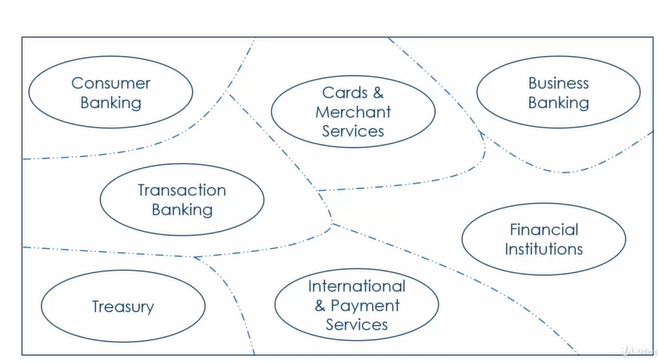
\includegraphics[scale = 1]{pictures/boi_canh_gioi_han/main.png}

    \caption{Ví dụ về bối cảnh bị giới hạn trong một ngân hàng}

\end{figure}

\subsubsection{Cách xác định bối cảnh bị giới hạn}

Để có thể xác định được bối cảnh bị giới hạn chúng ta có thể xem xét:

\begin{itemize}

    \item Dựa vào việc phân chia các miền phụ.

    \item Dựa vào sơ đồ cấu trúc tổ chức các phòng ban của doanh nghiệp.

    \item Dựa vào modules của các ứng dụng kiến trúc nguyên khối (nếu việc phân chia tốt).

    \item Dựa vào trách nhiệm và hoạt động của chuyên gia miền .

\end{itemize}

% \subsubsection{Áp dụng xác định bối cảnh bị giới hạn trong đồ án này}

% \subsubsection{Áp dụng xác định bối cảnh bị giới hạn trong đồ án này}

% \subsubsection{Áp dụng xác định bối cảnh bị giới hạn trong đồ án này}

% \subsubsection{Áp dụng xác định bối cảnh bị giới hạn trong đồ án này}

% \subsubsection{Áp dụng xác định bối cảnh bị giới hạn trong đồ án này}

% \subsubsection{Áp dụng xác định bối cảnh bị giới hạn trong đồ án này}

% \subsubsection{Áp dụng xác định bối cảnh bị giới hạn trong đồ án này}

% \subsubsection{Áp dụng xác định bối cảnh bị giới hạn trong đồ án này}

% \subsubsection{Áp dụng xác định bối cảnh bị giới hạn trong đồ án này}

% \subsubsection{Áp dụng xác định bối cảnh bị giới hạn trong đồ án này}

% \subsubsection{Áp dụng xác định bối cảnh bị giới hạn trong đồ án này}

% \subsubsection{Áp dụng xác định bối cảnh bị giới hạn trong đồ án này}

%!<! - - Hướng dẫn 5/10 - - >

%!<! - - Hướng dẫn 5/10 - - >

%!<! - - Hướng dẫn 5/10 - - >

%!<! - - Hướng dẫn 5/10 - - >

%!<! - - Hướng dẫn 5/10 - - >

%!<! - - Hướng dẫn 5/10 - - >

%!<! - - Hướng dẫn 5/10 - - >

%!<! - - Hướng dẫn 5/10 - - >

%!<! - - Hướng dẫn 5/10 - - >


\end{document}

\subsection{Miền dịch vụ (Service Domain)}

\chapter{Một số công nghệ trong kiến trúc vi dịch vụ}

%%%%%%%%%%%%%%%%%%%%%%%%%%%%%%%%%%
Bluider
Adapter
hẽagon củ hành
command CQRS

\end{document} % Kết thúc

% kết luận, tài liệu tham khảo

% \bibliographystyle{plain}
% \bibliography{references}
%%%%%%%%%%%%%%%%%%%%%%%%%%%%%%%%%%
% % phải có CQRS (Phân chia trách nhiệm truy vấn lệnh)

% CQRS là một mẫu kiến trúc riêng biệt có thể được sử dụng kết hợp với thiết kế hướng miền để đạt được những lợi ích nhất định, chẳng hạn như cải thiện hiệu suất và khả năng mở rộng. Tuy nhiên, nó không phải là một yêu cầu để triển khai thiết kế hướng miền.

% % phải có event

% Cách tiếp cận này nhấn mạnh tính mô - đun, tính linh hoạt và khả năng phục hồi, cho phép các nhóm làm việc đồng thời trên các phần khác nhau của hệ thống và cho phép phát hành nhanh hơn và thường xuyên hơn. Các vi dịch vụ thường dựa vào các giao thức truyền thông nhẹ, chẳng hạn như REST và thường được triển khai bằng các công nghệ chứa trong bộ chứa như Docker và Kubernetes.

% \subsubsection{DevOps Ứng dụng, áp dụng, liên quan, ....}

% \subsubsection{Github}

% \subsubsection{CI/CD}

% \subsubsection{Docker}

% \subsubsection{Kubernetes}

% dícovery

% % api gateway

% Repository độc lập miền và lưu trữ sql (dễ tuhaajn tiện Unit testing and Mocking)

% Repository trong ORM

% <!--https: //images.viblo.asia/fd4b10a0-f1b1-4ed1-9bd1-578c871820ae.png-->

%, gprc rabitmq đồng bộ hay k, ít hay nhiều như pub sub

% # 5. Service Mesh, CICD, microfe, API gateway, log xử lí lỗi,

% Bảng CSDL này được em thu thập dữ liệu từ trang web CƠ SỞ DỮU DANH MỤC DÙNG CHUNG (https: //dmdc.mof.gov.vn/khai-thac-pb/co-quan-thue)

% Chỉ dùng 1 loại hóa đơn vì em thấy tương tự.

% Loại hóa đơn: + Hóa đơn giá trị gia tăng + Hóa đơn bán hàng + Hóa đơn bán tài sản công + Hóa đơn bán hàng dự trữ quốc gia + Hóa đơn khác + Chứng từ điện tử được sử dụng và quản lý như hóa đơn

% <!--Các công nghệ phổ biến trong kiến trúc vi dịch vụ-->
% <!--RxJS-->
% https: //www.youtube.com/watch? v=6jSk_J7RA24
% https: //www.youtube.com/watch? v=Jc-lGeDuphg
% https: //www.youtube.com/watch? v=UXHzxX4png0
% https: //www.youtube.com/watch? v=glZs4QFfwbc

% # 7. Broker Pattern dịch vụ dicovery

% https: //www.youtube.com/watch? v=UXHzxX4png0

% # 8. Dependency Injection

% # 9. Kết luận tổng kết

% Kiến trúc vi dịch vụ, với việc tách biệt hệ thống thành các thành phần nhỏ quản lý độc lập, mang lại tính linh hoạt và khả năng mở rộng.

% thiết kế hướng miền giúp xây dựng mô hình chính xác và nhất quán của lĩnh vực kinh doanh, giúp đảm bảo rằng hệ thống phản ánh đúng yêu cầu nghiệp vụ.

% <!--@============================================== -->

% <!--@saga -->

% <!--@saga -->

% <!--@saga -->
% <!--@CQRS (Command Query Responsibility Segregation): -->

% <!--CQRS, EventSourcing, Sagas-->

% <!--@Event Sourcing: -->

% <!-- Strong Consistency : https://ddd-practitioners.com/?page_id=421 -->

% <!-- Snapshots : https://ddd-practitioners.com/snapshots -->

% <!-- Saga : https://ddd-practitioners.com/home/glossary/saga -->

% <!-- Outbox Pattern -->

% <!-- Optimistic Concurrency Control : https://ddd-practitioners.com/?page_id=609 -->

% <!-- https://www.linkedin.com/pulse/api-strategy-conways-law-inverse-conway-manoeuvre-mikael-wall%C3%A9n/ -->

% Một mô hình lưu trữ dữ liệu, trong đó tất cả các thay đổi trạng thái của hệ thống được biểu diễn dưới dạng sự kiện (event).

% <!-- EventStorming : https://ddd-practitioners.com/home/glossary/eventstorming -->

% <!-- Domain Storytelling : https://ddd-practitioners.com/?page_id=1005 -->

% <!-- CQRS : https://ddd-practitioners.com/?page_id=574 -->

% CQRS chia để thoải mái, chặt chẽ

% Là một nguyên tắc trong DDD, CQRS tách biệt giữa phần xử lý câu lệnh (Command) và phần truy vấn dữ liệu (Query).

% Command đại diện cho các thao tác cập nhật dữ liệu, trong khi Query đại diện cho các thao tác truy vấn dữ liệu.

% <!-- Event-Driven Architecture : https://ddd-practitioners.com/home/glossary/event-driven-architecture -->

% <!-- Event Modeling : https://ddd-practitioners.com/?page_id=994 -->

% <!-- Event Replay : https://ddd-practitioners.com/?page_id=585 -->

% <!-- Event Sourced Aggregates : https://ddd-practitioners.com/event-sourcing -->

% <!-- Event Sourcing : https://ddd-practitioners.com/?page_id=581 -->

% <!-- Eventual Consistency : https://ddd-practitioners.com/?page_id=419 -->

% <!-- Change Data Capture: https://en.wikipedia.org/wiki/CAP_theorem -->

% <!-- ACID Transaction : https://ddd-practitioners.com/?page_id=415 -->

% ACID (Atomicity, Consistency, Isolation, Durability)

% <!-- BASE Transaction -->

% BASE là viết tắt của "Basically Available, Soft state, Eventually consistent, " và đối lập với ACID

% <!-- Command : https://ddd-practitioners.com/?page_id=596 -->

% <!-- Command Handler : https://ddd-practitioners.com/?page_id=599 -->

% <!-- Compensating Action : https://ddd-practitioners.com/compensating-action -->

% <!-- Compensating Transaction : https://ddd-practitioners.com/compensating-transaction -->

% <!-- Compensating Workflow : https://ddd-practitioners.com/compensating-workflow -->

% <!-- Domain Event : https://ddd-practitioners.com/domain-event -->

% <!--@ Dependency Inversion Principle -->

% SOLID : https://ddd-practitioners.com/home/glossary/solid

% Single Responsibility Principle : https://ddd-practitioners.com/single-responsibility-principle

% Open-Closed Principle

% Liskov Substitution Principle : https://ddd-practitioners.com/home/glossary/liskov-substitution-principle

% Interface Segregation Principle : https://ddd-practitioners.com/?page_id=817

% <!--!========================================================== -->

% <!-- mỗi dịch vụ xuất bản và đăng ký các sự kiện nếu cần. Cách tiếp cận này có thể mở rộng và linh hoạt hơn so với điều phối, nhưng cũng phức tạp hơn trong việc triển khai và bảo trì. Tuy nhiên, nó cũng có thể linh hoạt hơn vì mỗi dịch vụ có thể phát triển độc lập và lỗi trong một dịch vụ không nhất thiết ảnh hưởng đến toàn bộ hệ thống. -->

% <!-- PublishSubscribe : https://www.enterpriseintegrationpatterns.com/patterns/messaging/PublishSubscribeChannel.html -->

% <!--@gRPC -->

% <!--@gRPC -->

% <!--@gRPC -->

% % Để phát triển tốt

% % cần tạo một bộ kiểm thử tích hợp tự động

% CI/CD đã trình bày bên trên

% % nhằm kiểm tra tính đúng đắn

% % %! Test - Driven Development : https:// thiết kế hướng miền - practitioners.com/test - driven - development

% % %! Test - Driven Development : https:// thiết kế hướng miền - practitioners.com/test - driven - development

% % %! Test - Driven Development : https:// thiết kế hướng miền - practitioners.com/test - driven - development

% % %! Test - Driven Development : https:// thiết kế hướng miền - practitioners.com/test - driven - development

% % %! Test - Driven Development : https:// thiết kế hướng miền - practitioners.com/test - driven - development

% [[Test - Driven Development]] TDD is a lightweight programming methodology that emphasizes fast, incremental development and especially writing tests before writing code. Ideally these follow one another in cycles measured in minutes. (see full definition under [[Test - Driven Development]] topic)

% Trang chủTrang chủBảng chú giảiHướng phát triển thử nghiệm

% Hướng phát triển thử nghiệm

% Phát triển dựa trên thử nghiệm (TDD) là một phương pháp phát triển phần mềm trong đó các thử nghiệm được viết trước khi mã thực tế được phát triển. Mục đích của TDD là đảm bảo rằng mỗi đoạn mã đều được kiểm tra đầy đủ và đáp ứng các yêu cầu của doanh nghiệp. TDD liên quan đến việc viết một bài kiểm tra thất bại trước tiên, viết mã vừa đủ để vượt qua, sau đó tái cấu trúc mã để cải thiện thiết kế của nó trong khi vẫn đảm bảo rằng tất cả các bài kiểm tra đều vượt qua.

% TDD là một phương pháp quan trọng trong Thiết kế hướng miền (thiết kế hướng miền) vì nó giúp đảm bảo rằng mã được phát triển phù hợp với mô hình miền và các quy tắc miền. Bằng cách viết bài kiểm tra trước, nhà phát triển buộc phải suy nghĩ về mô hình miền và các quy tắc miền trước khi viết bất kỳ mã nào. Các thử nghiệm trở thành một cách để xác định hành vi của hệ thống và giúp tập trung vào các yêu cầu kinh doanh. Khi mã được phát triển và tái cấu trúc, các thử nghiệm sẽ đảm bảo rằng hệ thống vẫn phù hợp với mô hình miền và các yêu cầu kinh doanh.

% % %! Test - Driven Development : https:// thiết kế hướng miền - practitioners.com/test - driven - development

% % %! Test - Driven Development : https:// thiết kế hướng miền - practitioners.com/test - driven - development

% % %! Test - Driven Development : https:// thiết kế hướng miền - practitioners.com/test - driven - development

% % %! Test - Driven Development : https:// thiết kế hướng miền - practitioners.com/test - driven - development